%Version 3 October 2023!
% See section 11 of the User Manual for version history
%
%%%%%%%%%%%%%%%%%%%%%%%%%%%%%%%%%%%%%%%%%%%%%%%%%%%%%%%%%%%%%%%%%%%%%%
%%                                                                 %%
%% Please do not use \input{...} to include other tex files.       %%
%% Submit your LaTeX manuscript as one .tex document.              %%
%%                                                                 %%
%% All additional figures and files should be attached             %%
%% separately and not embedded in the \TeX\ document itself.       %%
%%                                                                 %%
%%%%%%%%%%%%%%%%%%%%%%%%%%%%%%%%%%%%%%%%%%%%%%%%%%%%%%%%%%%%%%%%%%%%%

%%\documentclass[referee,sn-basic]{sn-jnl}% referee option is meant for double line spacing

%%=======================================================%%
%% to print line numbers in the margin use lineno option %%
%%=======================================================%%

%%\documentclass[lineno,sn-basic]{sn-jnl}% Basic Springer Nature Reference Style/Chemistry Reference Style

%%======================================================%%
%% to compile with pdflatex/xelatex use pdflatex option %%
%%======================================================%%

%%\documentclass[pdflatex,sn-basic]{sn-jnl}% Basic Springer Nature Reference Style/Chemistry Reference Style


%%Note: the following reference styles support Namedate and Numbered referencing. By default the style follows the most common style. To switch between the options you can add or remove ``Numbered'' in the optional parenthesis. 
%%The option is available for: sn-basic.bst, sn-vancouver.bst, sn-chicago.bst%  
 
%%\documentclass[sn-nature]{sn-jnl}% Style for submissions to Nature Portfolio journals
%%\documentclass[sn-basic]{sn-jnl}% Basic Springer Nature Reference Style/Chemistry Reference Style
\documentclass[pdflatex,sn-mathphys-num]{sn-jnl}% Math and Physical Sciences Numbered Reference Style 
%%\documentclass[sn-mathphys-ay]{sn-jnl}% Math and Physical Sciences Author Year Reference Style
%%\documentclass[sn-aps]{sn-jnl}% American Physical Society (APS) Reference Style
%%\documentclass[sn-vancouver,Numbered]{sn-jnl}% Vancouver Reference Style
%%\documentclass[sn-apa]{sn-jnl}% APA Reference Style 
%%\documentclass[sn-chicago]{sn-jnl}% Chicago-based Humanities Reference Style

%%%% Standard Packages
%%<additional latex packages if required can be included here>

\usepackage{graphicx}%
\usepackage{multirow}%
\usepackage{amsmath,amssymb,amsfonts}%
\usepackage{amsthm}%
\usepackage{mathrsfs}%
\usepackage[title]{appendix}%
\usepackage{xcolor}%
\usepackage{textcomp}%
\usepackage{manyfoot}%
\usepackage{booktabs}%
\usepackage{algorithm}%
\usepackage{algorithmicx}%
\usepackage{algpseudocode}%
\usepackage{listings}%
\usepackage{bm}
\usepackage{macros}
\usepackage{float}% For H placement specifier to force figure position
\usepackage{caption}% For caption control and \captionof command
\usepackage{afterpage}

%%%%

%%%%%=============================================================================%%%%
%%%%  Remarks: This template is provided to aid authors with the preparation
%%%%  of original research articles intended for submission to journals published 
%%%%  by Springer Nature. The guidance has been prepared in partnership with 
%%%%  production teams to conform to Springer Nature technical requirements. 
%%%%  Editorial and presentation requirements differ among journal portfolios and 
%%%%  research disciplines. You may find sections in this template are irrelevant 
%%%%  to your work and are empowered to omit any such section if allowed by the 
%%%%  journal you intend to submit to. The submission guidelines and policies 
%%%%  of the journal take precedence. A detailed User Manual is available in the 
%%%%  template package for technical guidance.
%%%%%=============================================================================%%%%

%% as per the requirement new theorem styles can be included as shown below
% \theoremstyle{thmstyleone}%
\theoremstyle{plain}%
\newtheorem{theorem}{Theorem}%  meant for continuous numbers
%%\newtheorem{theorem}{Theorem}[section]% meant for sectionwise numbers
%% optional argument [theorem] produces theorem numbering sequence instead of independent numbers for Proposition
\newtheorem{proposition}[theorem]{Proposition}% 
%%\newtheorem{proposition}{Proposition}% to get separate numbers for theorem and proposition etc.

\theoremstyle{thmstyletwo}%
\newtheorem{example}{Example}%
\newtheorem{remark}{Remark}%

\theoremstyle{thmstylethree}%
\newtheorem{definition}{Definition}%

\raggedbottom
%%\unnumbered% uncomment this for unnumbered level heads

\begin{document}

\title{Decoding Fossil Floras with Artificial Intelligence}
% \title{Identifying fossil leaves to family using deep neural networks: example from the Florissant flora}
\author[1]{\fnm{Ivan Felipe} \sur{Rodriguez}}
\equalcont{These authors contributed equally to this work.}

\author[1,2]{\fnm{Thomas} \sur{Fel}}
\equalcont{These authors contributed equally to this work.}

\author[1]{\fnm{Gaurav} \sur{Gaonkar}}
% \equalcont{These authors contributed equally to this work.}

\author[1]{\fnm{Mohit} \sur{Vaishnav}}

\author[3]{\fnm{Herbert} \sur{Meyer}}

\author[4]{\fnm{Peter} \sur{Wilf}}

\author*[1]{\fnm{Thomas} \sur{Serre}}\email{thomas\_serre@brown.edu}

\affil*[1]{\orgdiv{Department of Cognitive and Psychological Sciences}, \orgname{Brown University}, \orgaddress{ \city{Providence},  \state{Rhode Island}, \country{USA}}}

\affil[2]{\orgdiv{Kempner Institute}, \orgname{Harvard University}, \orgaddress{ \city{Boston}, \state{Massachusetts}, \country{USA}}}

\affil[3]{\orgdiv{Florissant Fossil Beds National Monument}, \orgname{National Park Service}, \orgaddress{ \city{Florissant},  \state{Colorado}, \country{USA}}}

\affil[4]{\orgdiv{Department of Geosciences}, \orgname{Pennsylvania State University}, \orgaddress{ \city{University Park 16802},  \state{Pennsylvania}, \country{USA}}}

%% Suggested author list: Rodriguez* Fel* Gonkar Vaishnav Meyer Wilf** Serre**
% Just a proposal. Let me (TS) know if you disagree. Also anybody that I forgot?

\abstract{
Accurately identifying fossil angiosperm leaves remains one of paleobotany's most persistent 
challenges. Although the morphological complexity of leaves has historically hindered manual 
classification, artificial intelligence (AI) is well-suited to extracting subtle diagnostic patterns 
that elude human perception. However, applying standard AI approaches to fossil material faces 
a fundamental limitation: the extreme scarcity of taxonomically vetted fossil specimens precludes 
conventional supervised training at scale. While modern leaf specimens are abundant, fossilization 
processes---compression, mineralization, fragmentation---create a challenging domain shift between 
living and fossil forms.

Here, we introduce a deep learning framework that overcomes this challenge by augmenting sparse 
fossil data with synthetic examples and aligning extant and fossil leaf domains through 
representational learning. Our approach synthesizes high-fidelity fossil analogs from modern leaf 
images (cleared and X-rayed) and trains a deep neural network using multi-scale representations that capture features ranging from 
fine venation patterns to overall leaf morphology, with triplet-loss embedding to align the two domains. 
We evaluate the system on the late Eocene Florissant flora of Colorado, achieving a top-5 F1-score 
of 91.8\% (chance: 3.5\% across 142 families) for family-level classification of fossil leaves. 
Remarkably, the system maintains a 73.4\% F1-score even when fossil families are entirely excluded from 
training---demonstrating robust out-of-distribution generalization. To interpret the model's decision 
process, we developed concept-based dictionary learning methods that identify and localize visual 
features driving classification decisions. We demonstrate practical utility by applying our system 
to 1,723 previously unidentified leaf fossils from the Florissant Formation, providing predictions 
with visual explanations to guide expert review. 

By overcoming data scarcity through generative AI and representational learning, this work offers a 
pathway to unlocking large-scale paleobotanical ``dark data''---the vast collections of unidentified 
specimens in museum drawers worldwide.
}
\maketitle


\section*{Introduction}
Isolated leaves dominate the angiosperm fossil record yet remain notoriously difficult to identify accurately, representing paleobotany's largely untapped source of ``dark data''~\cite{Dilcher_1971}. Historical literature is riddled with botanically incorrect identifications due to the inherent complexity of leaf morphology, insufficient vetted reference samples, and considerable variation within and across fossil sites. Consequently, most well-identified fossil leaves represent only a handful of morphologically distinctive families that are well-represented in the literature, leaving the vast majority of angiosperm diversity in the fossil record unrecognized~\cite{Hickey1975, Wilf2008FossilLeaves}. Accurate fossil leaf classification is crucial because leaf fossils provide essential data for interpreting evolutionary radiations and extinctions, biome evolution, plant-animal interactions, biogeography, and biotic responses to climate change~\cite{Giraldo2025, Hickey1977, Johnson1989, Kooyman2014, Wing2005}. At the family level---the traditional first step for most extant and fossil plant identifications---classification provides a stable taxonomic anchor, since nearly all fossil plants represent extinct species and many belong to extinct genera. Our previous work demonstrated that computer vision algorithms can generalize morphological features of leaves at this level~\cite{wilf2016leaves}.

Artificial intelligence (AI) shows promise for automating plant and palynomorph identification~\cite{plantclassificationGunjal2024,machinelearningspecies,Adaime2024}, but it faces the same fundamental limitations as human experts: small labeled datasets and strong site-to-site taphonomic variation. Overcoming these challenges requires both improved modeling of leaf morphology and strategies to augment scarce fossil data. To control for taphonomic variability, we focus here on a single, exceptionally well-documented fossil locality---the late Eocene Florissant Fossil Beds National Monument in Colorado. Preserved under relatively consistent lacustrine conditions~\cite{Harding2000}, the Florissant flora represents one of the best-understood Cenozoic plant assemblages, first described in MacGinitie's seminal 1953 monograph~\cite{mcginitie1953fossil} and subsequently expanded and revised through decades of systematic research~\cite{manchester1983fagopsis,Manchester2001Florissant,Jia2014Cercis,Herendeen2019Arcoa}.

Herb Meyer's digital archive~\cite{florissant}, recently recompiled as part of a large open-access dataset of fossil, cleared, and X-rayed leaves totaling more than 34,000 images~\cite{Wilf2024LeafDatasetV2}, provides a uniquely rich and accessible foundation for AI applications in paleobotany. From this resource, we curated 3,200 taxonomically vetted Florissant fossil leaves spanning 23 plant families (16 families with $\geq$5 specimens each). An additional 1,723 Florissant specimens lacking confident family assignments under modern standards were reserved to test the predictive validity of our models.

% Full-page Figure 1
\begin{figure}[p]
    \centering
    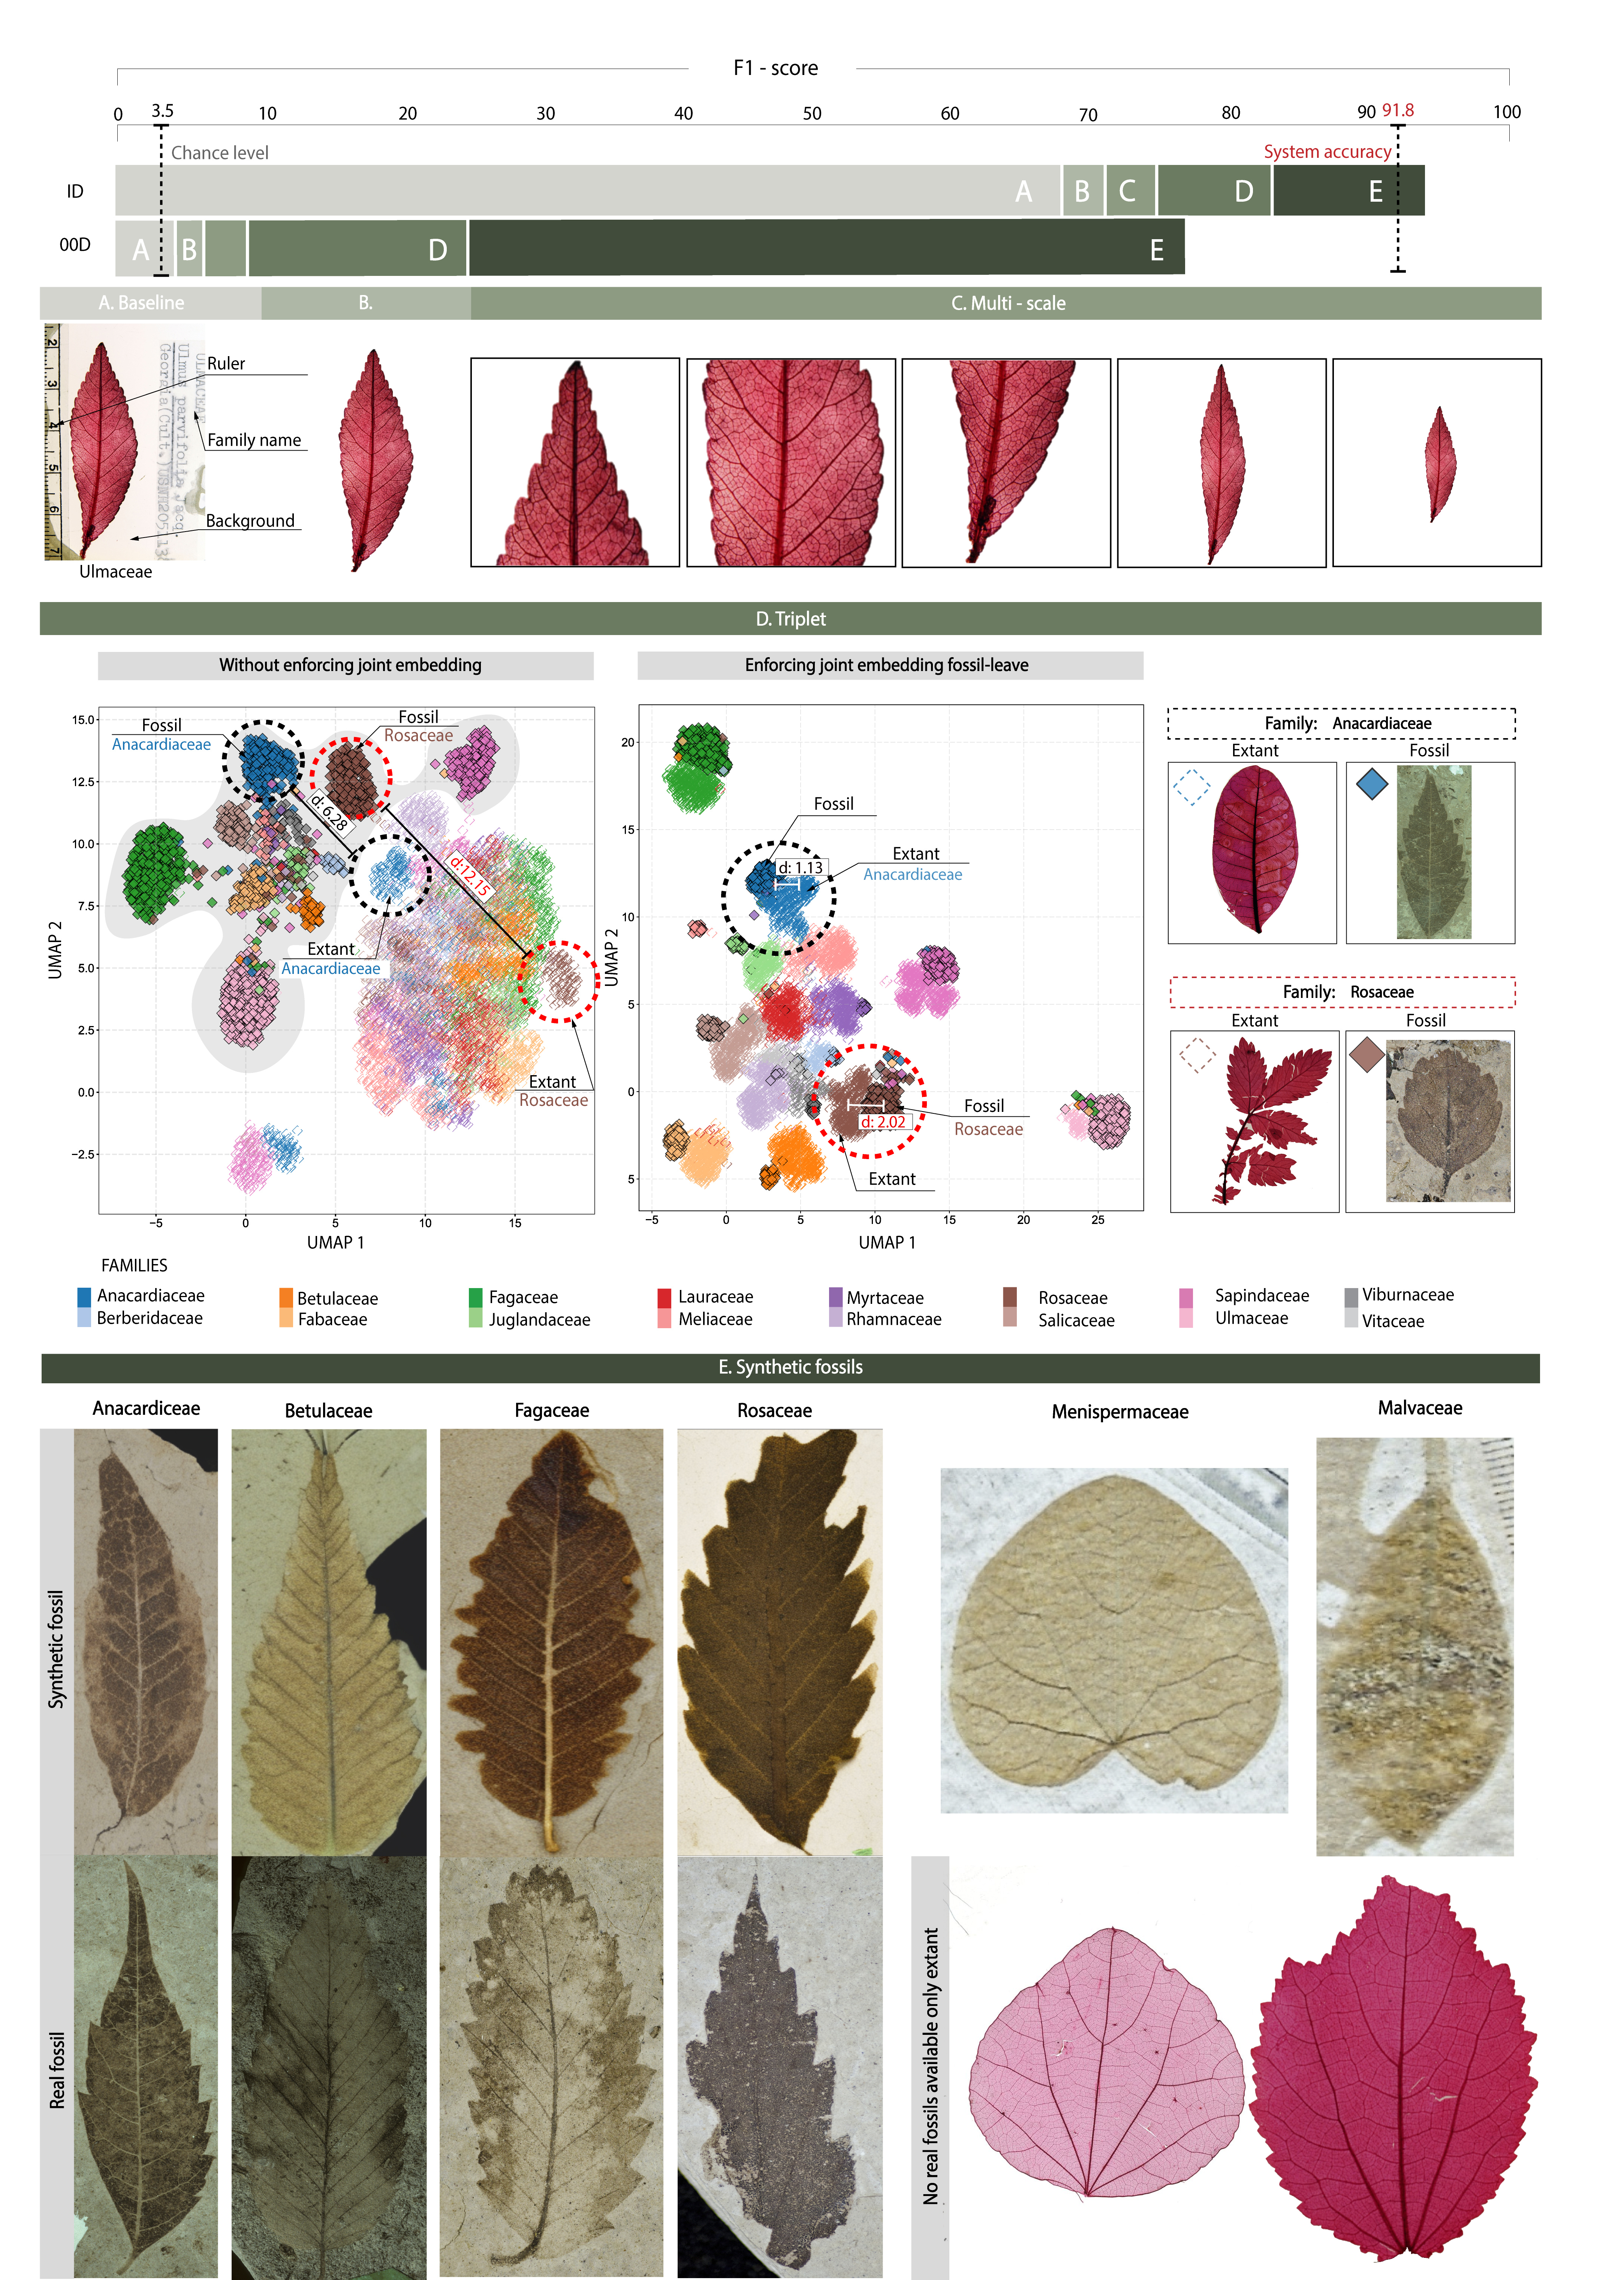
\includegraphics[width=\textwidth,height=0.95\textheight,keepaspectratio]{Figures/Figure_1_v8.png}
\end{figure}

\clearpage

% Caption for Figure 1 on the next page
\noindent\captionof{figure}{
Overview of system improvements for fossil leaf family identification and their cumulative impact on classification accuracy. 
\textbf{Top:} Top-5 $F_1$-scores for two generalization scenarios --- \textbf{in-distribution (ID)}, where real fossils were included during training, and \textbf{out-of-distribution (OOD)}, where only synthetic fossils were used. The dashed line marks the 3.5\% chance level for 142 families. The final model achieves 91.8\% accuracy across extant and fossil leaves. 
\textbf{Panels A--E:} 
(\textbf{A}) Baseline --- raw extant leaf image. 
(\textbf{B}) Segmentation --- background and artifacts (e.g., ruler, text) removed to ensure the model focuses on leaf morphology. 
(\textbf{C}) Multi-scale learning --- each leaf is analyzed at five resolutions to capture both overall shape and fine venation patterns. 
(\textbf{D}) Triplet loss embedding --- enforces a shared representation between fossil and extant leaves of the same family: (left) without alignment, clusters separate by domain; (right) with triplet loss, clusters group by family. 
(\textbf{E}) Synthetic fossils --- photorealistic fossil images generated to augment families with few or no real fossils. Examples show synthetic fossils (top), real fossils (bottom), and the corresponding extant leaves used as references when real fossils are unavailable.
}
\label{fig:system}

A central obstacle for fossil classification is that many families have few or no vetted fossil training exemplars. To address this, we employ a generative domain-translation approach to synthesize fossil-like images from extant cleared and X-rayed leaves. Specifically, a cycle-consistent, ControlNet-based model~\citep{zhang2023adding} is trained to translate images from 142 modern families (each with $\geq$25 specimens) into fossil-like versions, while using vetted Florissant fossils from 16 families to anchor the mapping between extant and fossil domains. This approach effectively expands the number of families represented in the fossil domain and substantially increases the diversity of training material. The classifier is trained jointly on (i) extant cleared and X-rayed leaves, (ii) real Florissant fossils where available, and (iii) synthetic fossil images generated by the domain translator. Incorporating these synthetic fossils markedly improves family-level accuracy and F1-score for both families with and without real fossil training samples, demonstrating that generative augmentation can overcome long-standing data scarcity in macrofossil paleobotany (Fig.~\ref{fig:system}).

\section*{Results}

We developed our deep learning architecture through multiple iterations and cumulative improvements using a ResNet-101 backbone~\cite{resnetHe2015}, a widely used 101-layer convolutional neural network with strong performance across computer vision tasks. Very similar results were obtained with a transformer architecture (See Supplementary Table~\ref{tab:beit}). Throughout this work, we report the top-5 F1-score of our deep learning model, i.e., the proportion of test images correctly classified when considering the model's top five predictions. We chose this metric because it is more informative than simple F1-score in a multi-class setting with 142 angiosperm families, where the top-5 predictions can be informative and exact match F1-score can underestimate performance. The chance-level performance for this classification task is 3.5\%. Importantly, we also evaluated model performance in terms of error rate and found that the results were qualitatively similar, supporting the robustness of our conclusions. All experiments used (80\%, 10\%, 10\%) train, validation, and test splits, respectively. We systematically tried different model settings (grid search) and selected the best using validation data. All F1-score measures reflect the model F1-score on the test set averaged across independent stratified random splits, $n = 10$.

Evaluating fossil-specific performance is challenging because vetted fossil specimens are available for only 16 of the 142 angiosperm families in our dataset. To quantify classification F1-score specifically for fossil leaves, we restricted our test set to these 16 families while the model still classified across all 142 families. For our baseline comparison, we used only real samples without any synthetic fossils. We evaluated two scenarios to establish performance bounds. In the \textbf{in-distribution (ID)} scenario, real fossil specimens from the test family were included during training, with evaluation performed on unseen real specimens of the same family using standard train/validation/test splits. This yielded an average test F1-score of 67.3\%, which constitutes the baseline F1 score for our architecture. 

In the more challenging \textbf{out-of-distribution (OOD)} scenario, we adopted a leave-one-family-out protocol where all real fossils from one family were withheld during training, and the model was tested on the complete set of real fossil leaves from that excluded family. As a baseline, we trained and tested only on real examples. This baseline OOD evaluation yielded an overall F1-score of 3.82\% on test fossils, reflecting the considerably greater difficulty of generalizing from extant cleared and X-rayed images to fossil leaf images (Fig.~\ref{fig:system}).

A common challenge in deep learning is the tendency for neural networks to rely on spurious correlations---so-called shortcuts---between image backgrounds and text annotations and class labels. This issue is particularly problematic in scientific applications, where hidden data acquisition biases, annotation artifacts such as handwriting patterns or label sizes, or preparation procedures can lead models to overfit to unintended cues rather than meaningful biological features~\citep{Brown2023ShortcutTesting,Nauta2022SkinShortcut,Hill2024ShortcutRisk}. 




To assess the robustness of our model against such shortcuts, we computed attribution maps using saliency methods from our custom Xplique toolbox~\citep{fel2022xplique}. Visual inspection revealed that the model sometimes based its decisions partly on background elements, potentially due to biases in how family labels were distributed across collections and variations in slide preparation. The model also leveraged annotations and text on slides as classification cues (see Fig.~\ref{fig:attribution_maps} for more details). Although these shortcuts might improve model ID F1-score, they most likely harm OOD generalization to novel collections and fossil specimens with different backgrounds.

To address this issue, we fine-tuned the Segment Anything Model (SAM)~\cite{kirillov2023segment} using 576 manually annotated, cleared leaf images, enabling effective leaf segmentation from their background. After applying this model to mask backgrounds across the entire dataset (Fig.~\ref{fig:system}), we confirmed that classification F1-score remained high (90.5\% for the whole system with small but robust improvements in our OOD (4.6\%) and ID (70.1\%) evaluations). Crucially, attribution maps showed that this new model predominantly relies on leaf morphology rather than background artifacts or manual annotations (Fig.~\ref{fig:attribution_maps}).


To further improve model performance, we hypothesized, according to standard understanding of leaf architecture \cite{Hickey1975}, that leaves encode diagnostic features across multiple spatial scales, from macroscopic traits such as overall shape and margin to mesoscopic patterns such as venation. To capture this morphological information, we extended our architecture to process images at multiple scales. Each input image was decomposed into five sub-images: the original masked image, a tighter crop defined by the smallest bounding box enclosing the leaf mask, and three additional crops corresponding to the basal, middle, and distal thirds of the leaf (Fig.~\ref{fig:system}). This multiscale approach improved classification F1-scores to 75.1\% (ID) and 8.72\% (OOD).



Fossil leaves often differ markedly from extant specimens due to damage, partial preservation, compression artifacts, and the surrounding rock matrix, which introduces variable background textures. We hypothesized that these differences might lead the model to treat extant and fossil leaves as distinct domains. To test this, we measured the average Euclidean distance between fossil and extant samples within each family in the model's embedding space, normalized by the average inter-family distance (see Fig.~\ref{fig:system}, Panel~D). This analysis showed that fossil and extant samples from the same family were substantially more distant in embedding space (\textit{mean normalized distance} = 11.45, SD = 3.1) than when the model was trained with a triplet loss to enforce cross-domain similarity (\textit{mean normalized distance} = 1.72, SE = 0.2). Because these embedding distances are dimensionless, they directly reflect representational dissimilarity within the neural network. A UMAP visualization of the penultimate-layer embeddings confirms this trend (Fig.~\ref{fig:system}, Panel~D, left), illustrating why general-purpose plant identification systems such as \textit{PlantNet} struggle to recognize fossil leaves.
 

To address the domain shift, we trained the model with an additional constraint that encourages it to bring leaves from the same family closer together in its internal representation, even when one is a fossil and the other is modern, while pushing apart leaves from different families. This approach (implemented with a triplet-loss; see Methods) explicitly shapes the embedding space so that fossil and extant leaves of the same family are aligned (Fig. \ref{fig:system}, Panel D, right). Incorporating this constraint substantially improved performance, reaching F1-scores of 82.3\% (ID) and 24.6\% (OOD), with the largest gains in the OOD scenario where vetted fossil examples were not available during training.
\begin{figure}[t!]
    \centering
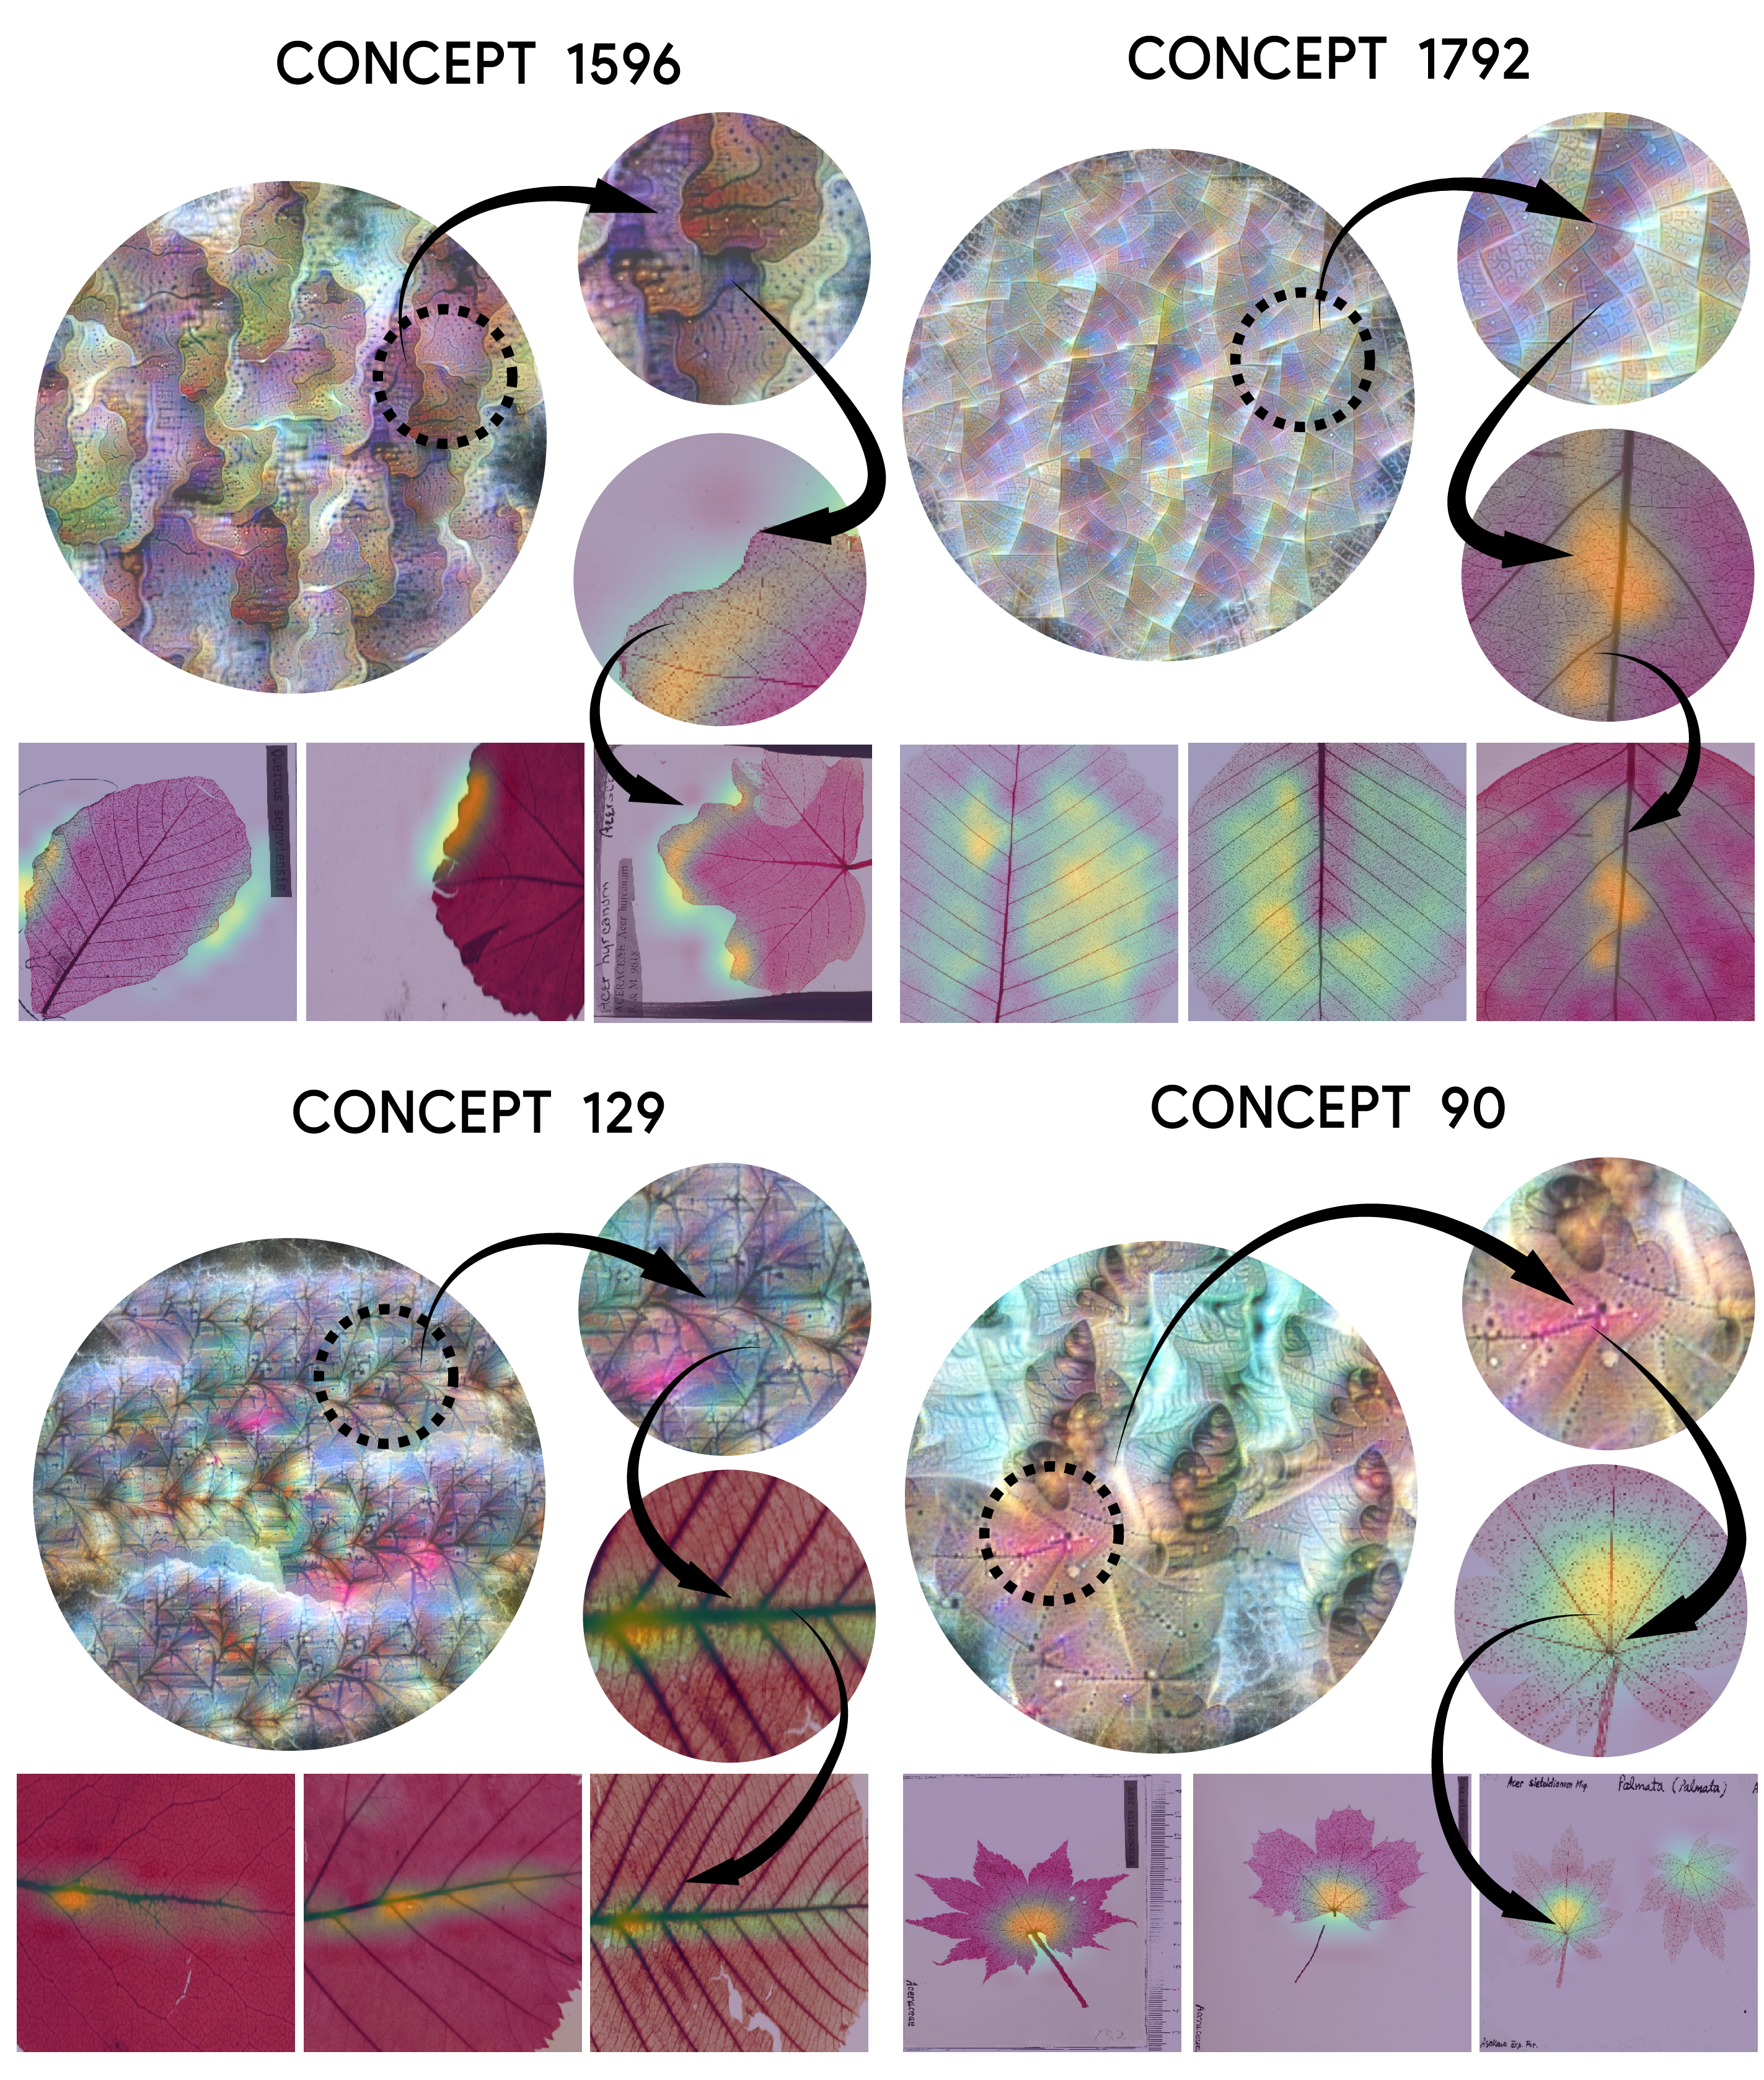
\includegraphics[width=.7\linewidth]{Figures/Figure_6_v2.jpg}
    \caption{Examples of visual ``concepts'' used by the model for classification. Concept 1596: active on the leaf margin. Concept 1792: active in intercostal areas. Concept 129: activates at junctions between primary and secondary veins. Concept 90: activates at leaf base. Additional examples shown in Fig.~\ref{fig:SI_concepts} and Fig.~\ref{fig:SI_concepts2}. Full set available at \url{https://fel-thomas.github.io/Leaf-Lens/}.} 
    \label{fig:concepts}
\end{figure}

A remaining challenge is the significant imbalance exhibited by our dataset, comprising 34,328 extant and 3,200 fossil leaves---approximately a 10:1 ratio. This problem is compounded by the complete absence of fossil specimens for most families in our dataset (119 of 142 families), with seven additional families having fewer than five samples. To address this limitation, we leveraged generative AI by adapting a stable diffusion model based on the ControlNet architecture~\citep{zhang2023adding}. Originally pre-trained on the LAION 5-billion image dataset, this conditional diffusion model synthesizes images guided by text prompts. We fine-tuned the network to generate realistic cleared leaf and fossil images, training it jointly with our ResNet-101 classifier using a combined objective that includes classification F1-score, triplet-loss alignment of extant and fossil representations within families, and the ControlNet loss (Methods). This generative data augmentation dramatically improved OOD generalization, raising OOD F1-score from near-chance levels (3.82\%) for our base model to 77.3\%, and from 67.4\% to 93.2\% (ID), substantially narrowing the performance gap between the two evaluation scenarios. 


High-performing AI models often function as black boxes, making the rationale behind their predictions difficult to interpret, even though, in the case of leaves, they contain abundant, novel taxonomic information~\cite{spagnuolo2022decoding, wilf2016computer}. To address this, we developed an explainability framework~\cite{fel2024sparks} to identify internal visual concepts utilized by our fossil-leaf classification model, potentially uncovering diagnostic patterns difficult for human observers to discern~\cite{spagnuolo2022decoding}. Specifically, our interpretability framework comprises three key stages: (\textbf{\textit{i}}) concept extraction, (\textbf{\textit{ii}}) importance estimation, and (\textbf{\textit{iii}}) concept visualization.

% First, we \emph{extract} a structured and interpretable sparse dictionary of visual concepts from the model's internal representations using a Top-\(k\) Sparse Autoencoder. This step is critical, as the internal feature space of deep neural networks often exhibits an overcomplete representation, with individual neurons encoding a superposition of multiple semantic factors. Direct analysis of raw activations could obscure this semantic structure, prompting us to employ sparse dictionary learning on intermediate-layer activations to derive a compact, disentangled set of visual primitives that the model relies upon~\cite{}.

% Second, we \emph{quantify} the importance of each extracted concept to the model's predictions. Rather than assigning equal weight to all concepts, we reparameterize the classifier in concept space, directly attributing the model's outputs to underlying concepts via a linear mapping. Each concept thus receives a class-specific importance score reflecting its influence on the decision boundary~\cite{}.

% Third, to make these concepts accessible and interpretable, we \emph{visualize} them spatially and semantically. Spatial visualization involves generating dense concept activation maps, clearly localizing concept activations within input images, while semantic visualization synthesizes prototypical input examples that selectively and maximally activate each concept~\cite{}. These three stages provide a structured, transparent decomposition of the model's internal reasoning, enhancing human interpretability and trust in model predictions.


% High-performing models often function as black boxes, making their decision-making rationale difficult to interpret. To address this, we developed an explainability framework to identify internal visual ``concepts'' utilized by our model, potentially uncovering diagnostic patterns difficult for human observers to discern~\cite{spagnuolo22}. Our interpretability framework comprises three key stages: \textbf{concept extraction}, \textbf{importance estimation}, and \textbf{concept visualization}.
\begin{figure}
    \centering
    \includegraphics[width=1\linewidth]{Figures/Figure_5_features.png}
    \caption{Sample of high-level features used by the model to perform classification. }
    \label{fig:high_level_features}
\end{figure}

First, we extracted a structured dictionary of visual ``concepts'' from the model's internal representations using a Top-k Sparse Autoencoder~\cite{gao2024scaling}. This step is critical because deep neural networks often suffer from the problem of polysemanticity~\cite{elhage2022superposition}, with individual model units encoding multiple ``semantic'' dimensions simultaneously. To reveal this latent structure, we employ sparse dictionary learning~\cite{mairal2014sparse,olshausen1996emergence,tosic2011dictionary} on the penultimate layer activations~\cite{fel2023holistic} to derive a compact, disentangled set of visual concepts. Representative examples of these visual concepts are shown in Fig.~\ref{fig:concepts} and Fig.~\ref{fig:high_level_features}. See Fig.~\ref{fig:SI_concepts} and Fig.~\ref{fig:SI_concepts2} for additional examples and \url{https://serre-lab.github.io/Lens/} for the full set.

Second, we quantified the importance of each extracted concept for the model predictions. Rather than treating all concepts equally, we reparameterized the classifier in concept space, directly attributing model outputs to underlying concepts via linear mapping~\cite{fel2023holistic}. Each concept, hence, receives a class-specific importance score reflecting its influence on the decision boundary.

Third, we visualized these concepts using feature visualization methods~\cite{olah2017feature,fel2023unlocking} in two ways to enhance interpretability: heat maps~\cite{zeiler2013visualizing,fong2017meaningful,petsiuk2018rise,fel2021sobol}, which indicate where individual concepts are activated within each image, and maximally exciting images, which reveal the visual patterns that most strongly activate each concept. Together, these stages provide a transparent decomposition of the model's internal reasoning, enhancing interpretability and trust in model predictions (see Fig.~\ref{fig:concepts}; also explore more concepts at \url{https://serre-lab.github.io/Lens/}). 


\begin{figure}[t!]\centering
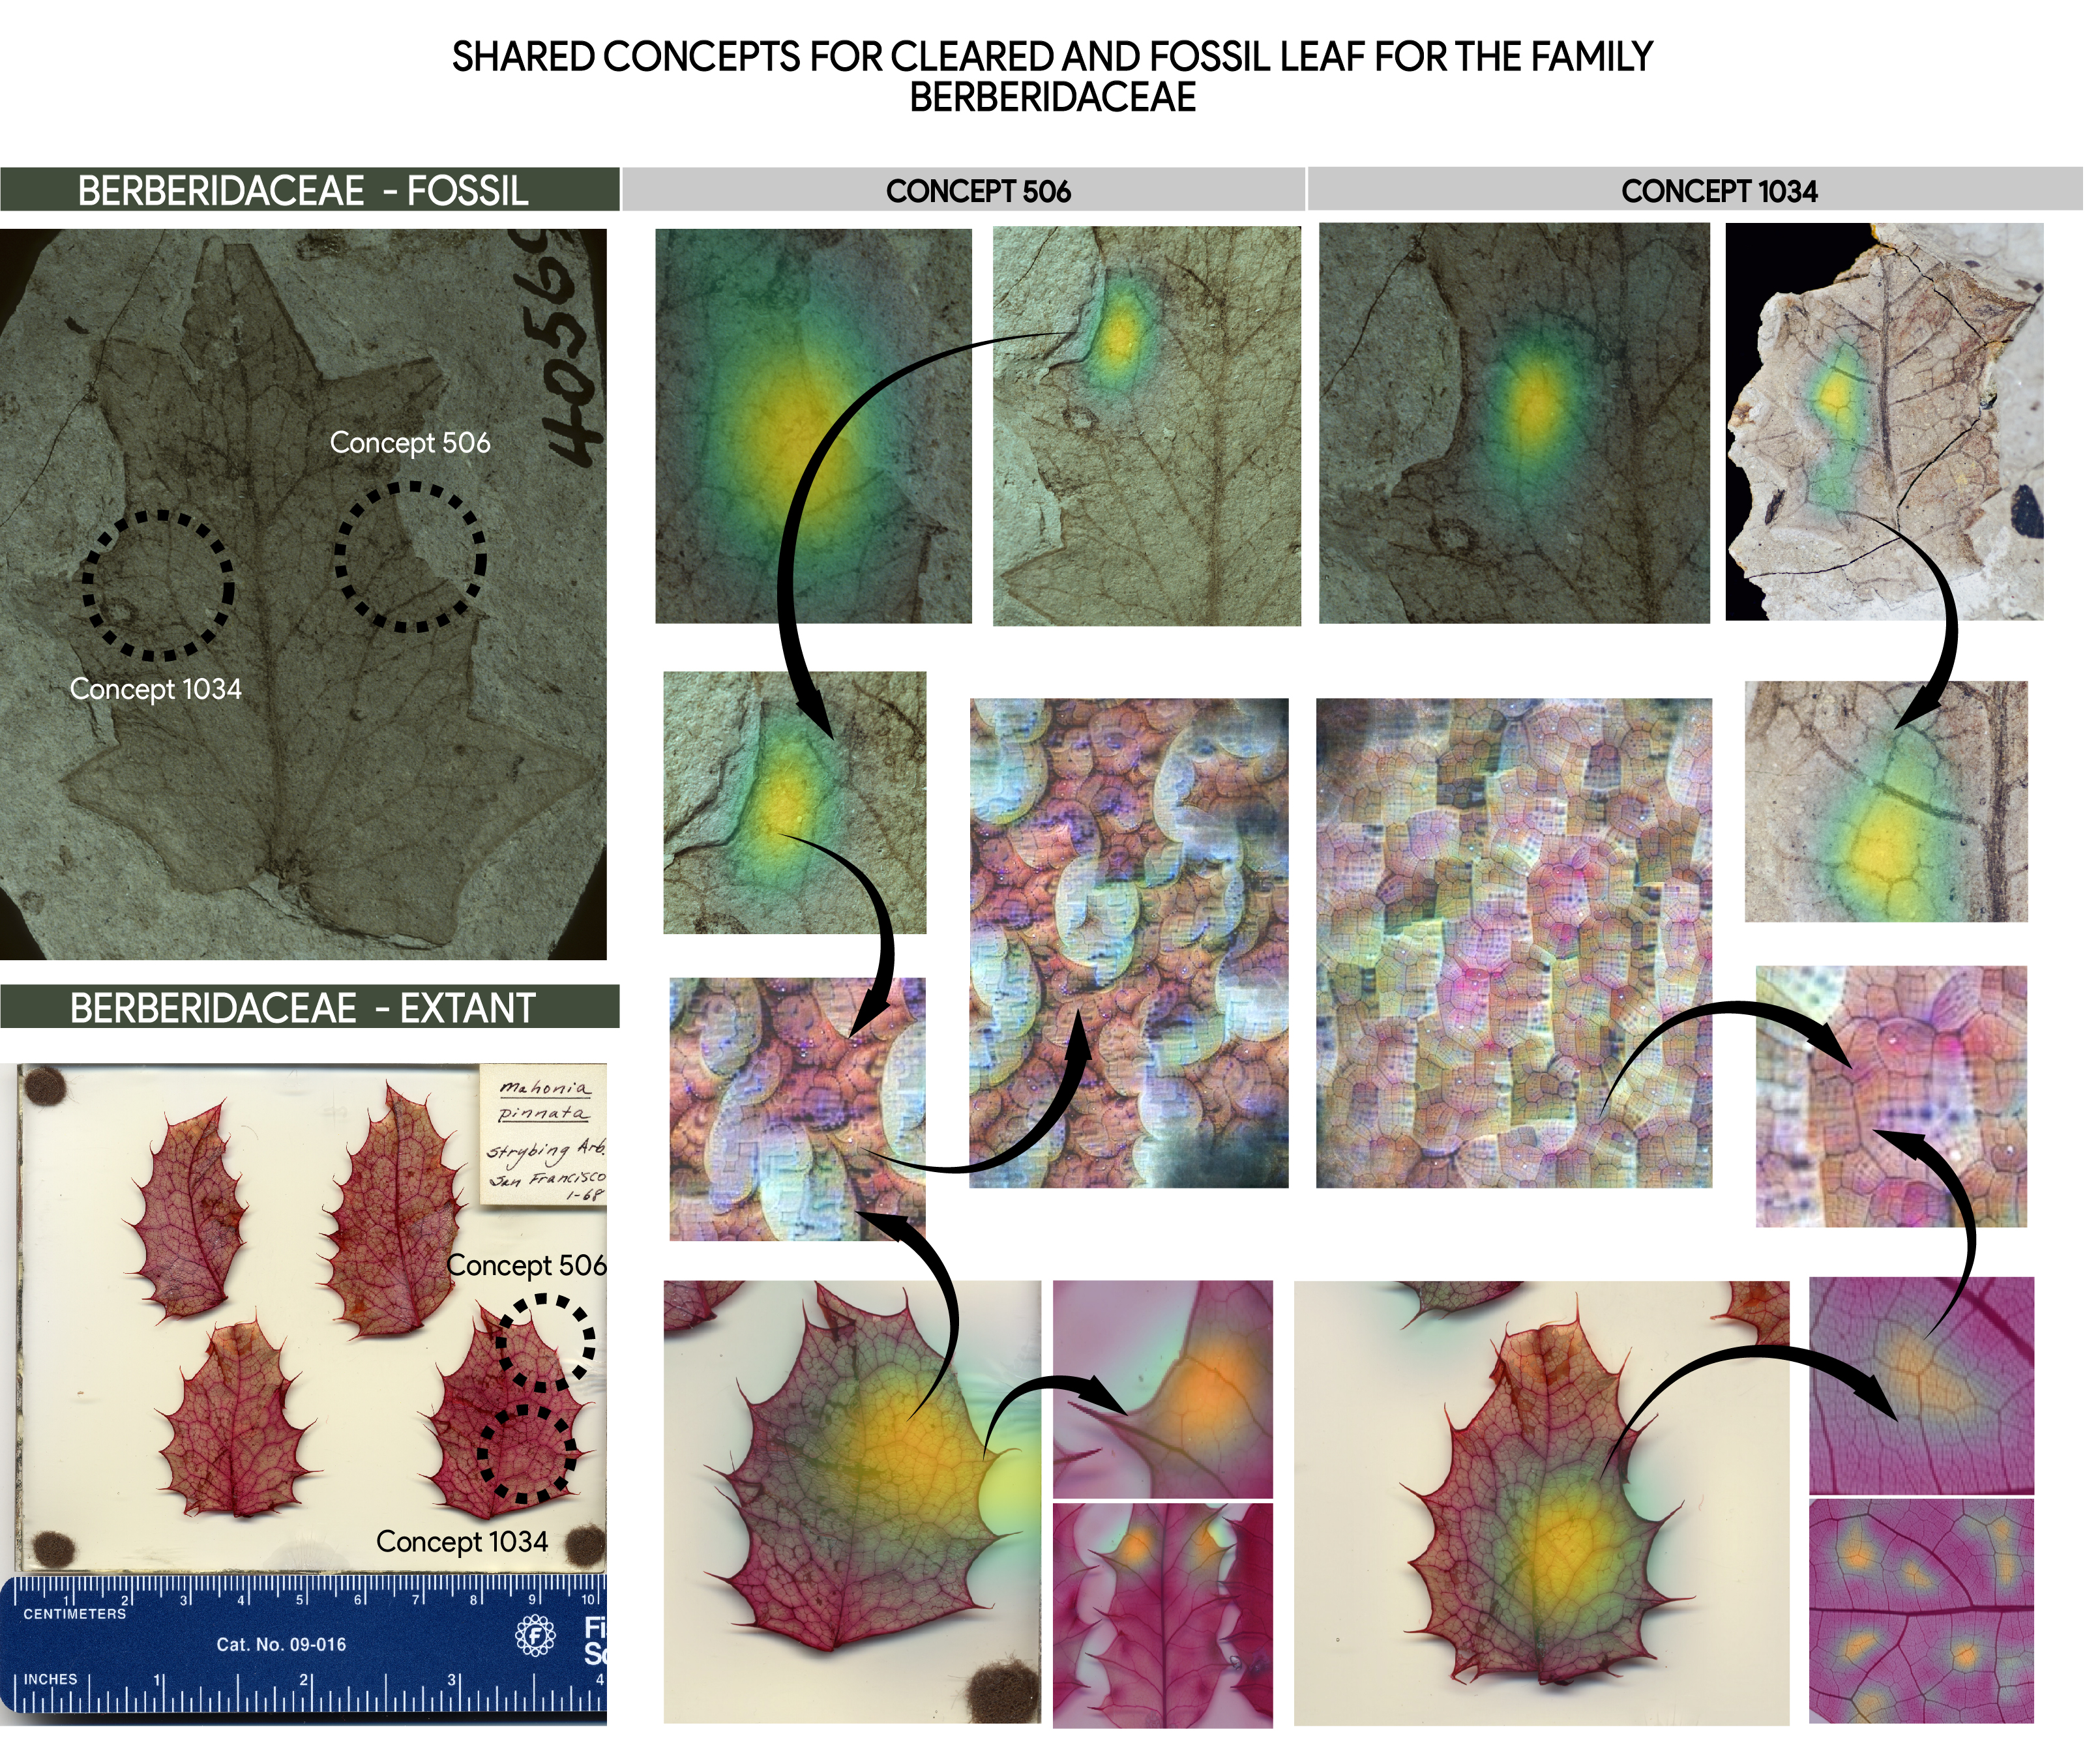
\includegraphics[width=.7\linewidth]{Figures/Figure_3_v3.jpg}
    \caption{Shared concepts used by the model to classify extant and fossil examples from the family Berberidaceae. }
    \label{fig:shared_concepts}
\end{figure}




\begin{figure}[t!]
    \centering
    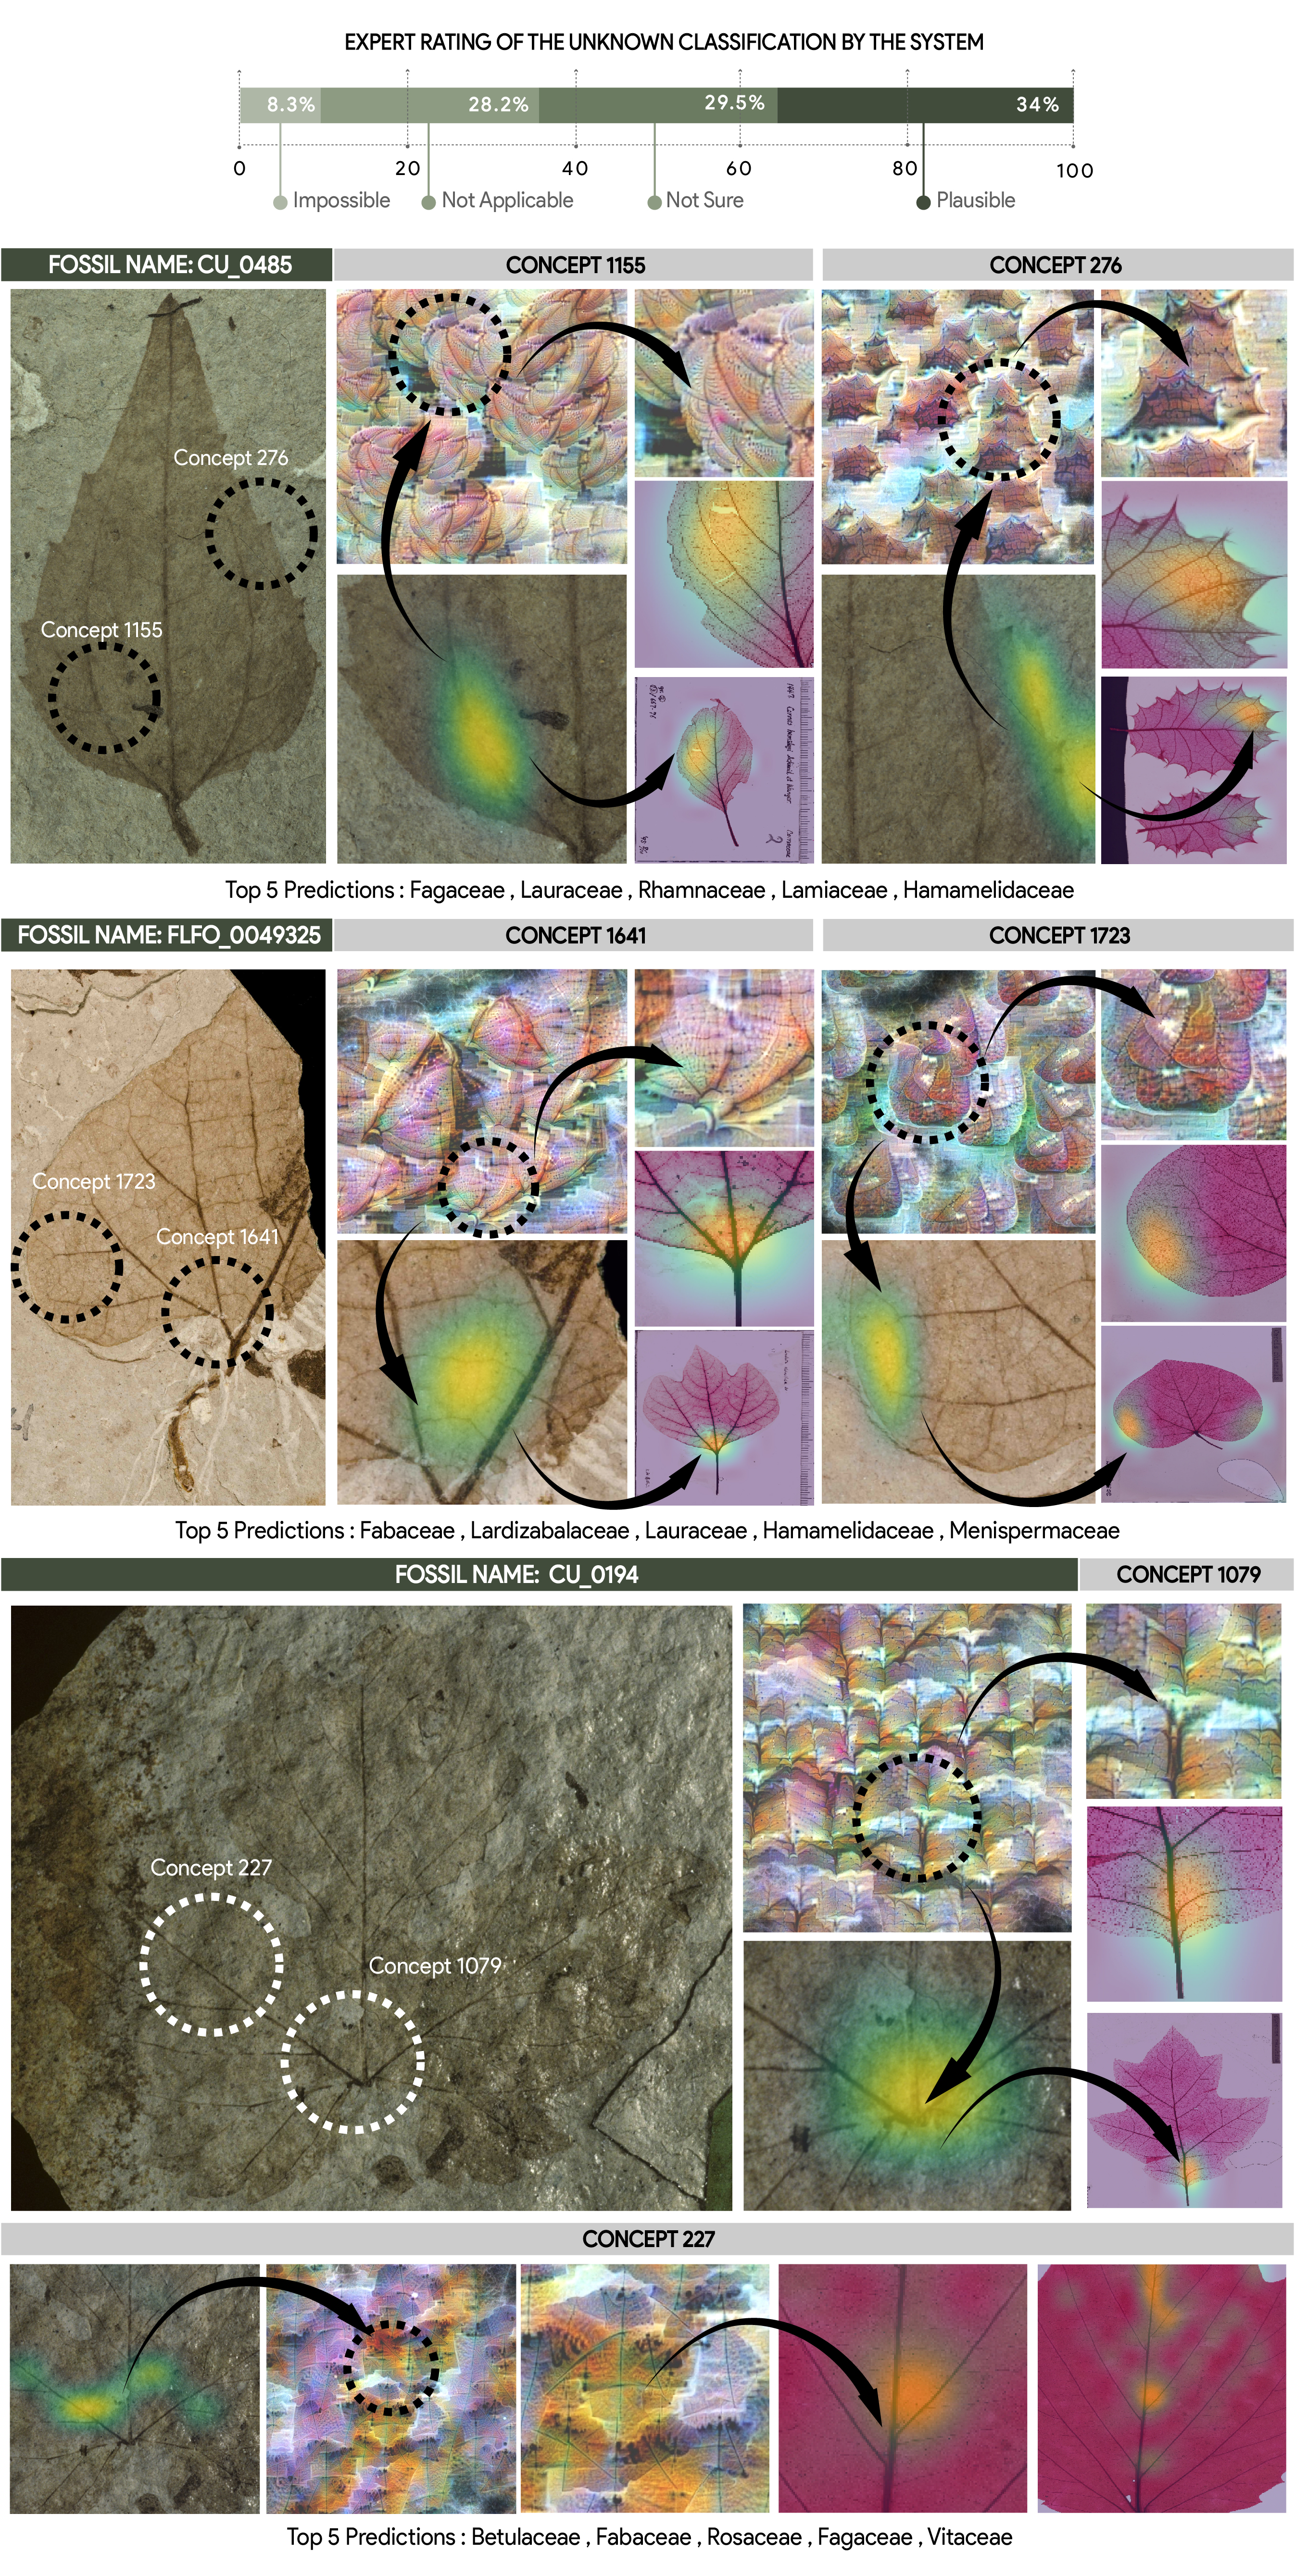
\includegraphics[width=0.9\linewidth]{Figures/Figure_2_v8.jpg}
  \caption{
\textbf{Top:} Expert evaluation of model predictions for previously unidentified Florissant fossils (categories: confident, plausible, uncertain, and not applicable). 
\textbf{Bottom:} Example unidentified fossils with the model's Top-5 family predictions and the most influential learned concepts (e.g., secondary-vein arrangement, marginal dentition, honeycomb-like areolation, and the junction of primary and secondary veins). 
The full set of predictions, visual explanations, and downloadable data are available at \url{https://serre-lab.github.io/prj_fossil_unknown/}.
}

    \label{fig:unknown}
\end{figure}
% \paragraph{Explainability}

\section*{Demo Application}

To broaden accessibility of our system, we developed an interactive web application available at \url{https://huggingface.co/spaces/Serrelab/fossil_app}. This demo enables users to upload fossil leaf images and obtain top family-level predictions generated by our model. In addition to classification results, the application provides saliency maps that visually highlight the regions of the leaf image most influential to the model's decision, offering an interpretable and user-friendly interface for exploring fossil leaf identification.




% To understand the decision-making process of our models, we employ explainability techniques such as Grad-CAM \cite{Selvaraju_2019} and RISE \cite{RISE2018} through the Xplique toolbox \cite{fel2022xplique}. These methods generate attribution maps highlighting the image regions that most influence predictions. 



% \begin{figure}[ht!]
%     \centering
%     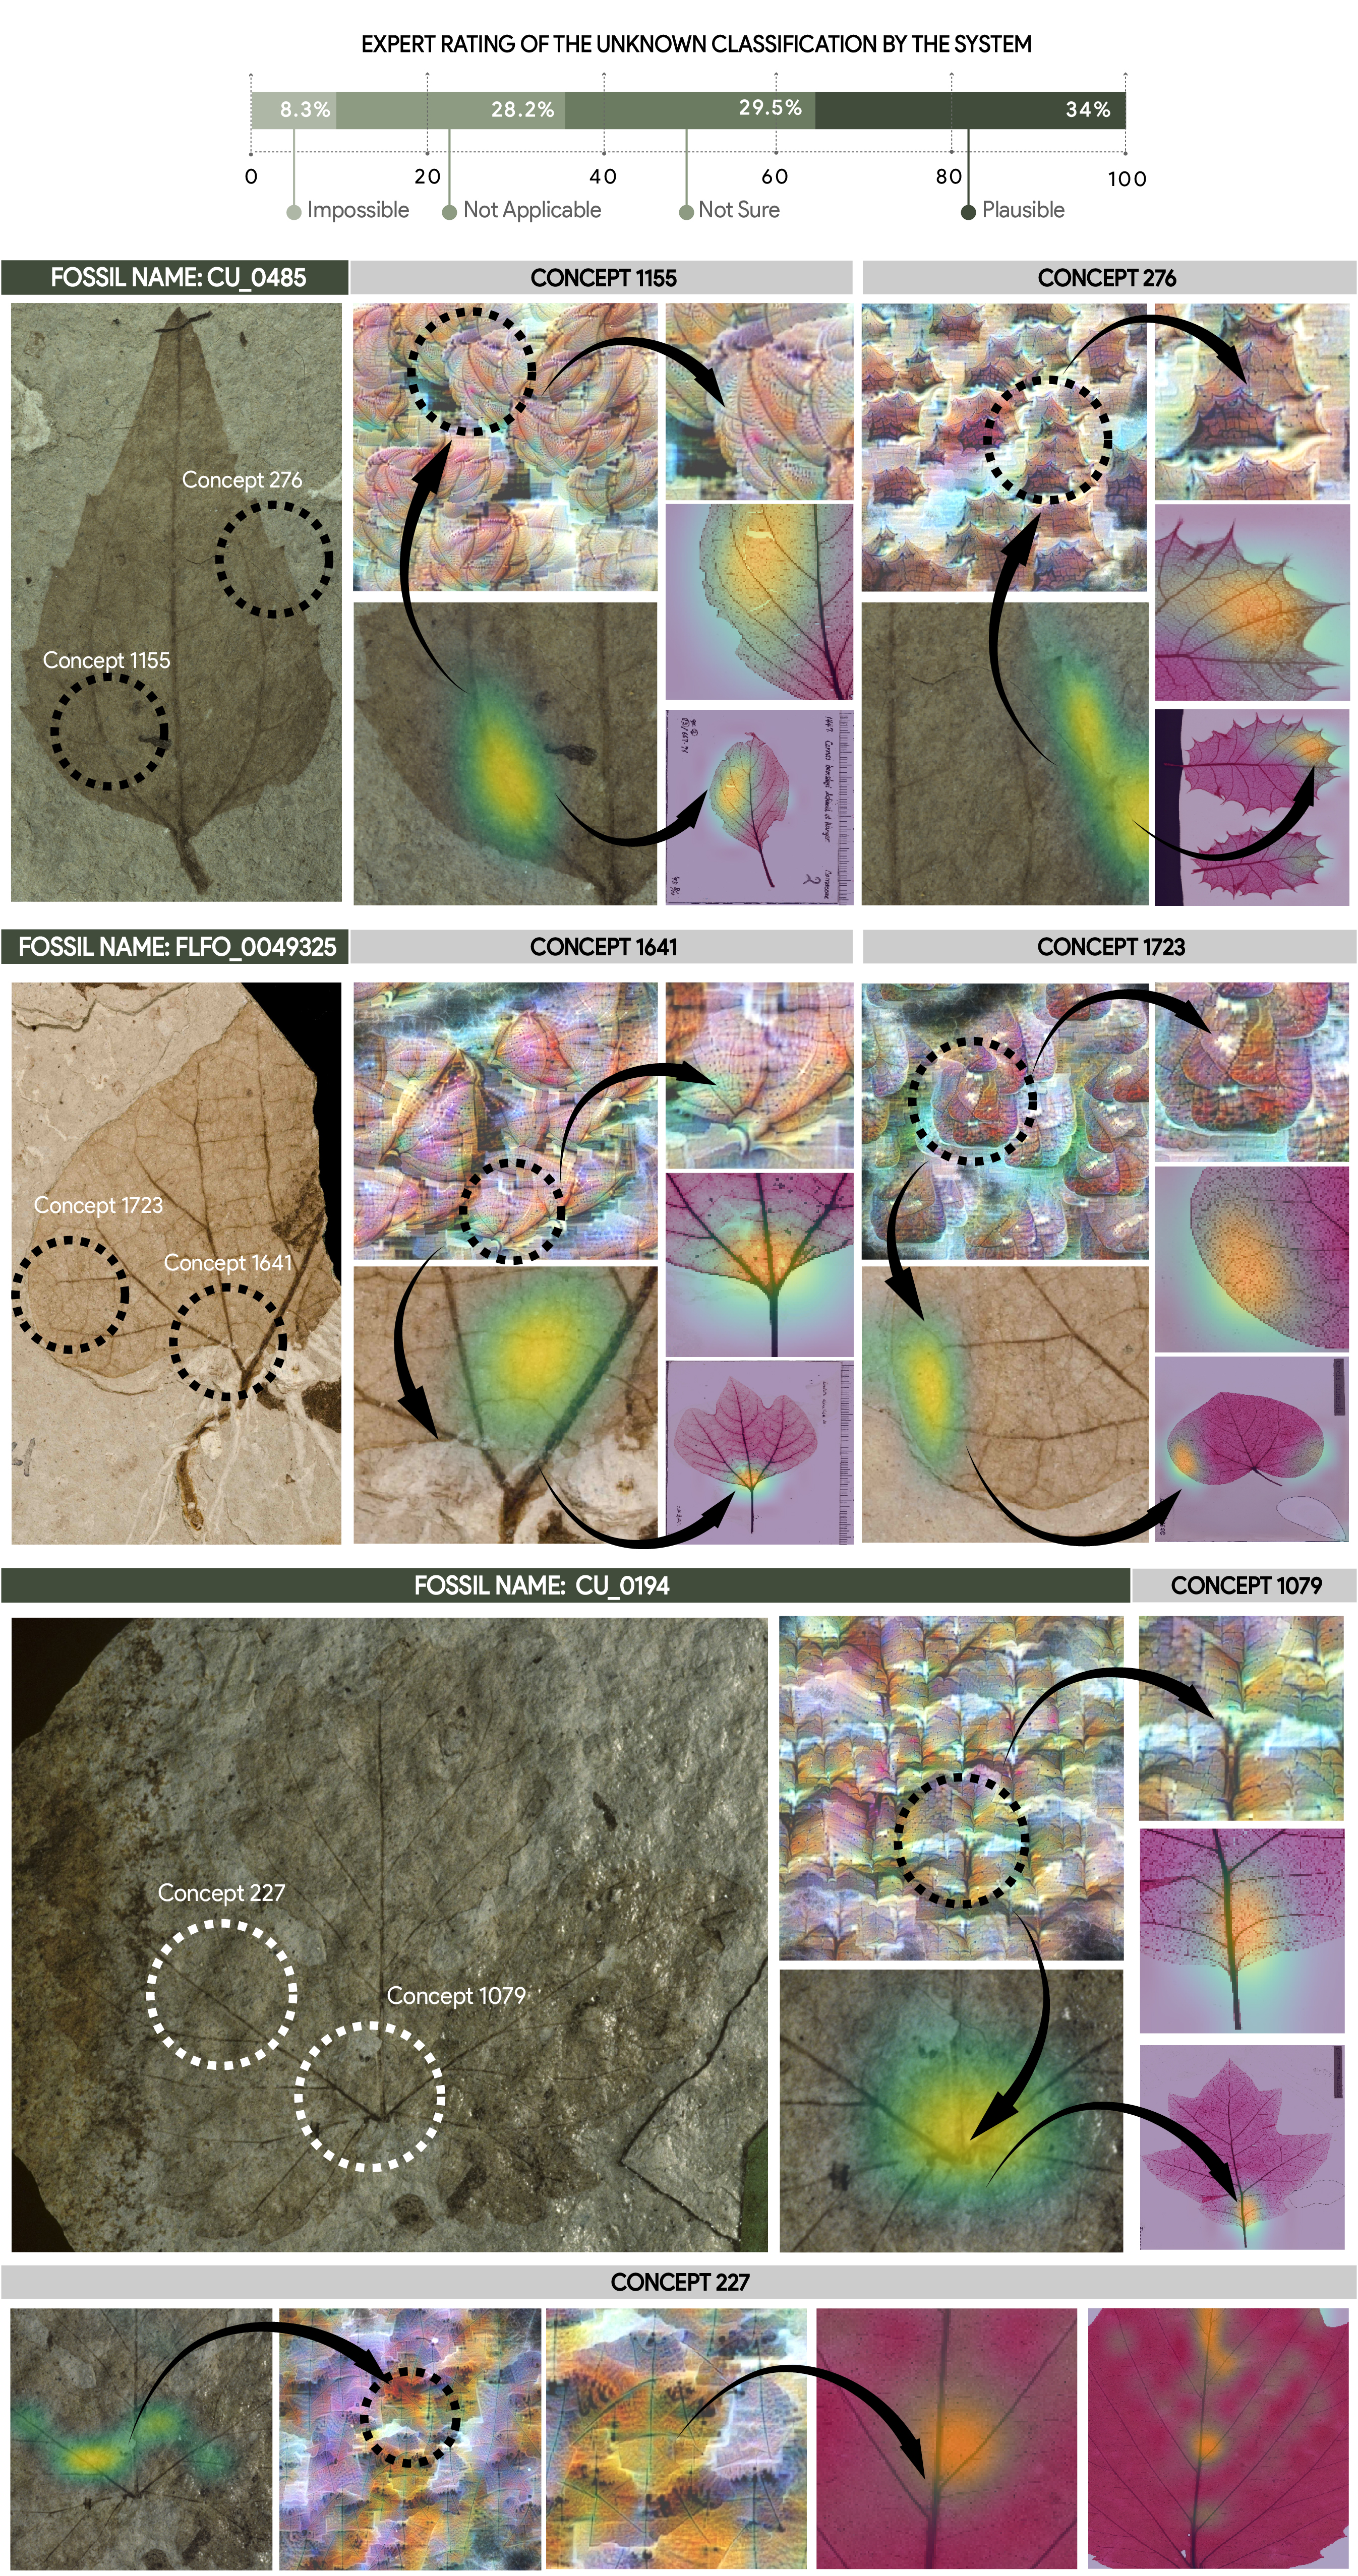
\includegraphics[width=\linewidth]{Figures/Figure_2_v7.jpg}
%     \caption{On top the distribution of the responses from the expert paleo-botanist evaluators. 8.3\% are predictions that are not possible, due to the fossil configuration. The  28.2\% of the fossils  were not applicable, meaning that their images were not properly taken and key features may have left out, or multiple leafs were present. 29.5\% are predictions that the expert are not sure and may constitute valuable cases were the concepts discovered by the system  can shed some light. 34\% of the cases were identified as plausible. The next row, there is an example of the Unidentified fossil, and the key concepts that were utilized for its classification, including the leaf formation on the left, the paternary vein in the middle and the junction between the paternary vein and the secondary veins.  }
%     \label{fig:system2}
% \end{figure}


Finally, we present the first machine-assisted classification of 1,723 fossil samples from the Florissant collection, encompassing specimens with previously unknown family labels or historical identifications no longer considered robust (see Fig.~\ref{fig:unknown}). These specimens came from the same sources as those in the vetted set \cite{Wilf2024LeafDatasetV2} but did not pass the vetting criteria. These correspond only to dicot angiosperm leaves (i.e., no monocot angiosperms due to very limited sample size).  The model's predictions and accompanying interpretability results were evaluated by the two team paleobotanists (P.W. and H.M.; Fig.~\ref{fig:unknown}). Their assessment revealed that 485 specimens (28.2\%) were either severely degraded, belonged to fossil categories other than dicot leaves, or lacked sufficient morphological detail for reliable human identification; these samples were therefore excluded from further evaluation. Among the remaining 1,238 specimens, the paleobotanists identified 585 classifications as intriguing and an additional 505 classifications as plausible, collectively representing promising candidates for detailed follow-up studies and offering abundant new opportunities for paleobotanical research on the Florissant flora. The experts found the model's predictions to be implausible for only 143 specimens (approximately 12\%), highlighting the system's robustness and potential utility for assisting paleobotanical classification tasks. An extensive list of specimens and computer annotations is available on our website \footnote{\url{https://serre-lab.github.io/prj_fossil_unknown/}}.  



\section*{Conclusion}
We present a robust framework that advances one of paleobotany's central challenges---accurate identification of fossil angiosperm leaves---and, importantly, ongoing cross-domain training and refinement promise broader applicability across diverse fossil sites, substantially extending its scientific impact. By harnessing modern generative AI to synthesize realistic fossil images from extant leaf data, our system attains high identification F1-scores even for families lacking fossil training examples. Using state-of-the-art interpretability methods, it also surfaces botanically meaningful cues by visually summarizing subtle morphological features that define families across fossil and extant specimens, suggesting new diagnostic characters.

Although our current model substantially improves the classification of previously unknown Florissant fossils, the same cross-domain strategy is readily generalizable to other deposits, positioning this approach for broad use. In the near term, it offers paleobotanists a practical, interpretable tool to reduce longstanding uncertainties in Florissant flora identifications and, more broadly, to advance our understanding of the evolution and ecological dynamics of ancient terrestrial ecosystems.


% In summary, We worked around the sample size limitations by successfully using synthetic fossils, resulting in correct identifications for families even when no fossil training data were available.
% State of the art visualization techniques provide novel botanical insights into the defining family-level characteristics seen in living and fossil leaves.
% Cross training and further development will allow expansion to include more fossil sites. 
% In the meantime, there is an immediate use case to improve identifications for the many Florissant unknowns.

% \paragraph{Segmentation and Preprocessing}
% \section*{Methods}

% \paragraph{Automated training dataset cleanup} 
% We fine-tune SAM on 500 manually annotated cleared leaf images using an 80/20 split, achieving a 95\% Intersection over Union (IOU). This fine-tuned model is then applied as a preprocessing step to segment the remainder of the dataset.  This segmentation not only removes artifacts but also ensures that the network focuses on intrinsic leaf morphology.

% \paragraph{Triplet loss}
% Following \cite{taha2020triplet}, our BEiT model is modified with two output heads: a classification head trained via cross-entropy loss and an embedding head optimized using triplet loss. For each class, we sample an anchor, a positive sample (same family), and a negative sample (different family) from the two domains, enforcing that the anchor-positive distance is minimized relative to the anchor-negative distance. The triplet loss is defined as:
% \begin{align}
%     \mathcal{L}_{trip} = \frac{1}{b} \sum_{i=1}^{b} \left[ D(a_{i,x}, p_{i,x}) - D(a_{i,x}, n_{i,x}) + m \right],
% \end{align}
% where \(b\) is the batch size, \(D\) is a distance function, \(a\) denotes the anchor, \(p\) the positive sample, \(n\) the negative sample, and \(m\) is a fixed margin. The overall loss is:
% \begin{equation}
%     \mathcal{L} = \mathcal{L}_{softmax} + \lambda \mathcal{L}_{trip}.
% \end{equation}
% Synthetic images generated from extant leaves are added to augment families with little or no fossil data. \textcolor{purple}{This design enforces both local and global structure in the embedding space, a key factor for robust classification when real fossil samples are limited.}

% \paragraph{Synthetic fossil generation}
% Let \(X\) denote the fossil domain and \(Y\) the extant (leaves) domain. Although they share certain morphological features, their visual properties differ substantially. In many cases, families represented in \(Y\) lack corresponding fossil samples in \(X\).

% Inspired by \cite{Zhu2017CycleGAN}, we adopt a generative approach. We define two mappings, \(G: X \rightarrow Y\) and \(F: Y \rightarrow X\), implemented as ControlNet modules \cite{Zhang2023ControlNet} with fixed random seeds. These modules are guided by text prompts:
% \begin{itemize}
%     \item ``A cleared leaf of the family: \textless Family Name\textgreater''
%     \item ``A fossilized leaf of the family: \textless Family Name\textgreater''
% \end{itemize}
% These prompts ensure that the generated images preserve family-specific traits. A triplet regularizer is used to enforce proximity among images of the same family across domains. Additionally, we apply SAM during generation to guarantee that the leaf shape remains consistent between the input and generated images.

\section*{Methods}

\paragraph{Families selected for this study}

The dataset used in this study comprises cleared and x-rayed images of specimens from the following dicot (non-monocot angiosperm) families: Acanthaceae, Achariaceae, Actinidiaceae, Altingiaceae, Amaranthaceae, Anacardiaceae, Annonaceae, Apiaceae, Apocynaceae, Aquifoliaceae, Araliaceae, Aristolochiaceae, Asteraceae, Atherospermataceae, Berberidaceae, Betulaceae, Bignoniaceae, Boraginaceae, Burseraceae, Buxaceae, Calophyllaceae, Calycanthaceae, Campanulaceae, Canellaceae, Cannabaceae, Capparaceae, Caprifoliaceae, Cardiopteridaceae, Celastraceae, Cercidiphyllaceae, Chloranthaceae, Chrysobalanaceae, Clusiaceae, Combretaceae, Connaraceae, Coriariaceae, Cornaceae, Crassulaceae, Cucurbitaceae, Cunoniaceae, Dilleniaceae, Dipterocarpaceae, Ebenaceae, Elaeagnaceae, Elaeocarpaceae, Ericaceae, Euphorbiaceae, Eupteleaceae, Fabaceae, Fagaceae, Flacourtiaceae, Garryaceae, Grossulariaceae, Hamamelidaceae, Icacinaceae, Iteaceae, Juglandaceae, Lauraceae, Lardizabalaceae, Lythraceae, Magnoliaceae, Malpighiaceae, Malvaceae, Melastomataceae, Meliaceae, Menispermaceae, Monimiaceae, Moraceae, Myristicaceae, Myrtaceae, Nyssaceae, Oleaceae, Papaveraceae, Passifloraceae, Phyllanthaceae, Pittosporaceae, Platanaceae, Polygonaceae, Proteaceae, Rhamnaceae, Rhizophoraceae, Rosaceae, Rubiaceae, Rutaceae, Salicaceae, Sapindaceae, Sapotaceae, Saxifragaceae, Schisandraceae, Simaroubaceae, Smilacaceae, Solanaceae, Staphyleaceae, Stemonuraceae, Symplocaceae, Tapisciaceae, Theaceae, Thymelaeaceae, Trochodendraceae, Ulmaceae, Urticaceae, Vitaceae,  and Winteraceae.

The families for which there were also fossil samples available are: Anacardiaceae, Berberidaceae, Betulaceae, Fabaceae, Fagaceae, Juglandaceae, Lauraceae, Meliaceae, Myrtaceae, Rhamnaceae, Rosaceae, Salicaceae, Sapindaceae, Ulmaceae, Viburnaceae,  and Vitaceae. 

\paragraph{Performance measures}
We evaluate our method using two distinct scenarios to establish in-distribution (ID) and out-of-distribution (OOD) bounds on performance:
\begin{enumerate}
    \item \textbf{ID scenario:} A standard 80/10/10 training/test/cross-validation where real fossils from each family are included in both training and testing sets.
    \item \textbf{OOD scenario:} A leave-one-family-out cross-validation, in which the training set excludes all real fossils from the test family (only fossils from the other families are included), and evaluation is performed solely on the withheld family.
\end{enumerate}

These scenarios provide robust estimates of ID (best-case) and OOD (worst-case) classification performance. 
Specifically, we report the F1-score, defined as:
\[
F_{1} = \frac{2 \cdot \text{Precision} \cdot \text{Recall}}{\text{Precision} + \text{Recall}} ,
\]
where $\text{Precision} = \frac{TP}{TP+FP}$ and $\text{Recall} = \frac{TP}{TP+FN}$ with $TP$, $FP$, and $FN$ denoting true positives, false positives, and false negatives, respectively. 

Additionally, we generated embedding visualizations with and without the triplet-loss regularizer, and performed qualitative analyses of attribution maps using Grad-CAM \cite{selvaraju2017gradcam} and RISE \cite{RISE2018} methods. These analyses further validated that our approach significantly enhances model interpretability and F1-score. Preliminary feedback from expert paleobotanists suggests that our method effectively highlights clear, family-specific visual features, thereby supporting the identification of previously unknown fossil specimens.


\paragraph{Automated training dataset cleanup} 
To ensure that our models rely exclusively on intrinsic leaf morphology rather than external artifacts, we fine-tuned the Segment Anything Model (SAM; \cite{kirillov2023segment}) on 576 manually annotated cleared-leaf images using an 80/20 training-validation split. The fine-tuned model achieved an Intersection over Union (IoU) of 95\%, demonstrating highly accurate segmentation performance. This segmentation model was subsequently applied to the entire dataset. Visual inspections revealed that the approach effectively removes background artifacts and annotations, thus encouraging the family classifier to focus solely on relevant morphological features.

\paragraph{Representation learning and triplet loss}
Building on~\cite{taha2020triplet}, we enhanced our classification architecture by adding a dedicated embedding head optimized with triplet-loss regularization alongside the standard cross-entropy classification head. For each training batch, we sample an anchor example with a positive (same-family) and a negative (different-family) using a hard sampling approach, meaning we picked the furthest positive and the closest negative (see Fig.~\ref{fig:SI_Full_system}) from both extant and fossil domains. The triplet loss encourages embeddings such that anchor-positive pairs are closer together than anchor-negative pairs by at least a margin \(m\). Formally, the triplet loss is defined as:
\begin{align}
    \mathcal{L}_{triplet} = \frac{1}{b} \sum_{i=1}^{b} \left[ D(a_{i,x}, p_{i,x}) - D(a_{i,x}, n_{i,x}) + m \right],
\end{align}
where \(b\) denotes batch size, \(m\) represents the margin, and \(x\) denotes the domain. \(D(\cdot)\) is a suitable distance metric, and \(a\), \(p\), and \(n\) represent anchor, positive, and negative samples, respectively. The combined objective function used during training is:
\begin{equation}
    \mathcal{L} = \mathcal{L}_{crossentropy} + \lambda \mathcal{L}_{triplet},
\end{equation}
where \(\lambda\) controls the relative contribution of the triplet loss. To further enhance robustness, synthetic fossil images generated from extant leaves were introduced to augment families with limited or absent fossil data. This strategy reinforces both local (within-family) and global (cross-family) structure within the embedding space, significantly improving model generalization, especially for families lacking representative fossil samples.

To quantitatively assess representational differences between the fossil and extant leaf domains and the impact of the triplet loss, we analyzed the learned embedding space by measuring how closely samples from the same family cluster together, regardless of whether they are extant or fossil. Specifically, for each family, we computed the average Euclidean distance between embeddings of extant and fossil leaves within that family (i.e., the ``intra-family, inter-domain'' distance). We then compared these ``intra-family, inter-domain'' distances to the average distance between embeddings from different families (``inter-family'' distances). To ensure comparability across families, we normalized the ``intra-family, inter-domain'' distances by the mean ``inter-family'' distance for each family. This normalization allows us to interpret the results as a relative measure: values less than one indicate that, on average, extant and fossil leaves from the same family are closer to each other in the embedding space than to leaves from other families. 

Our results show that, after applying the triplet loss, the normalized inter-domain, intra-family distances are substantially reduced, decreasing from an average of 11.45 with a standard deviation of 3.1 to an average of just 1.72 with a standard deviation of 0.3. This demonstrates that the model learns to align fossil and extant leaves from the same family in the embedding space, effectively bridging the domain gap. In other words, the triplet loss encourages the network to focus on family-level morphological features that are consistent across domains, rather than domain-specific artifacts. This effect is also visually apparent in the UMAP projection of the embeddings (Fig.~\ref{fig:system}), where fossil and extant leaves from the same family form tight, overlapping clusters.

\paragraph{Synthetic fossil generation}
Let \(X\) denote the fossil domain and \(Y\) the extant (cleared leaves) domain. While these domains share morphological characteristics, their visual appearance often differs substantially due to preservation conditions, artifacts, and inherent variability in fossilization. Furthermore, many families represented in domain \(Y\) lack corresponding fossil examples in domain \(X\).

To bridge this domain gap, we adopted a generative image-to-image translation approach inspired by CycleGAN~\cite{CycleGAN2017}, implemented using the ControlNet architecture~\cite{zhang2023adding}. Specifically, we defined two mappings, \(G: X \rightarrow Y\) (fossil-to-extant) and \(F: Y \rightarrow X\) (extant-to-fossil), each guided by domain-specific text prompts:
\begin{itemize}
    \item ``A cleared leaf of the family: \textless Family Name\textgreater''
    \item ``A fossilized leaf of the family: \textless Family Name\textgreater''
\end{itemize}
These text-based prompts guide ControlNet to generate synthetic images that preserve family-specific morphological features. Importantly, the generative model (ControlNet) and the classifier are trained together in an end-to-end fashion. The overall training loss is a weighted sum of the classification loss, the triplet loss, and the generative (ControlNet) loss, with all components optimized jointly during end-to-end training. This joint optimization ensures that the embeddings of both real and generated images are aligned within the same family across domains, and that the synthetic images produced are directly beneficial for the classification objective. At each training step, both the generator and classifier parameters are updated simultaneously, ensuring that synthetic fossil generation and classification performance are tightly coupled. 

Specifically,
\begin{equation}
    \mathcal{L}_{total} = \mathcal{L}_{classif} + \lambda_{trip} \mathcal{L}_{trip} + \lambda_{gen} \mathcal{L}_{gen}
\end{equation}
where $\mathcal{L}_{classif}$ is the standard classification loss, $\mathcal{L}_{triplet}$ is the triplet loss as defined above, $\mathcal{L}_{gen}$ is the generative loss for ControlNet, and $\lambda_{triplet}$ and $\lambda_{gen}$ are weighting coefficients for the triplet and generative losses, respectively.
Additionally, we applied the fine-tuned SAM model during synthetic image generation, ensuring that leaf shapes in synthetic images remain faithful to their input counterparts, thereby improving both visual realism and model generalization. Please find details for training in the SI. 



%%%%
\paragraph{Concept Extraction} We consider a dataset of input images $\X = \{ \x_i \}_{i=1}^n$, where $\x_i \in \R^{H \times W \times 3}$. Each image is processed by a visual encoder $\f$, yielding a latent feature tensor $\A_i = \f(\x_i) \in \R^{h \times w \times d}$, with spatial dimensions $(h, w)$ and feature dimension $d$. We aggregate activations across the dataset by flattening the spatial dimensions of each $\A_i$ and concatenating them into a global activation matrix $\A \in \R^{nhw \times d}$.

One might assume that meaningful visual concepts align with the $d$ coordinate axes (neurons) of the activation space, implying at most $d$ independently representable features. Yet this view underestimates the complexity of neural representations. Empirical findings indicate that, despite residing in a $d$-dimensional space, neural networks routinely encode many more than $d$ distinct features~\cite{ghorbani2019towards,fel2023craft,fel2023holistic}---a phenomenon referred to as superposition~\cite{elhage2022toymodelssuperposition}, which bears resemblance to a kind of distributed, compressed coding.

To put it simply, rather than relying on strictly orthogonal directions, as in conventional linear representations, the network appears to adopt a looser geometry, one in which directions are merely sufficiently decorrelated to permit reliable disambiguation. This strategy enables a form of representational overloading: distinct features are encoded along vectors that, while not strictly orthogonal, remain distinguishable within the tolerances of the task.

%This behavior finds a natural analogue in the Johnson--Lindenstrauss (JL) lemma~\cite{larsen2014johnson}, which guarantees that a collection of points in high-dimensional space can be projected into a lower-dimensional subspace while approximately preserving pairwise distances, provided that small distortions are admissible. Inverting this intuition, one arrives at a striking implication: if exact orthogonality is relaxed to $\varepsilon$-orthogonality, the number of nearly independent directions that can inhabit a $d$-dimensional space grows exponentially with $d$---up to $\mathcal{O}(\exp^d)$ under generous assumptions.
%
Given this understanding of the representation geometry of neural networks, overcomplete sparse dictionary learning~\cite{tovsic2011dictionary,rubinstein2010dictionaries,elad2010sparse,mairal2014sparse,dumitrescu2018dictionary,olshausen1997sparse,hurley2009comparing}~has emerged as a natural tool to reverse-engineer this geometry~\cite{cunningham2023sparse, bricken2023monosemanticity, rajamanoharan2024jumping, gao2024scaling, surkov2024unpacking, gorton2024missing, bhalla2024interpreting,fel2025archetypal}. Rather than assuming that concepts align with the original $d$ coordinate axes, we seek to discover a larger set of $c \gg d$ directions in the activation space, each corresponding to a semantically meaningful visual concept. Formally, we decompose the activation matrix $\A$ using a learned overcomplete dictionary $\D \in \R^{c \times d}$ and sparse coefficient matrix $\Z \in \R^{nhw \times c}$ by solving:
\begin{equation}
\min_{\Z, \D} \|\A - \Z\D\|_F^2 \quad \text{subject to} \quad \|\Z_i\|_0 \leq k, \quad \Z_i \geq 0, \quad \|\D_j\|_2 = 1 \quad \forall i, j \in [c]
\end{equation}
%where $\|\cdot\|_F$ denotes the Frobenius norm, the $\ell_0$ constraint enforces that each activation pattern uses at most $k$ concepts, non-negativity ensures additive interpretability, and unit-norm dictionary atoms $\D_j$ provide canonical concept directions.
The sparsity constraint is crucial: it reflects the empirical observation that while the model may have access to thousands of concepts, any given input activates only a small subset, consistent with the superposition hypothesis.
%
In practice, we implement this decomposition using a Top-$k$ Sparse Autoencoder~\cite{gao2024scaling,fel2025archetypal}. %which learns the dictionary through gradient descent while enforcing the structural constraints. 
The encoder applies a learned linear projection, followed by ReLU activation and a Top-$k$ sparsification operator $\bm{\Pi}_k(\cdot)$ that retains only the $k$ highest activations: $\Z = \bm{\Pi}_k(\text{ReLU}(\A\bm{W}_{\texttt{enc}}))$. The decoder reconstructs activations as $\hat{\A} = \Z\D$, where each dictionary atom $\D_j$ represents a distinct visual ``concept'' whose semantic meaning emerges through the optimization process. 
%This formulation transforms the black-box activation space into an interpretable concept space where complex visual patterns decompose into meaningful, additive components.

\paragraph{Concept Quantification}
Having decomposed the neural representation into interpretable concepts (see Fig.~\ref{fig:high_level_features}), we address the question of quantifying their individual contributions to model predictions. The sparse dictionary learning framework yields a linear reparameterization that renders explicit the relationship between concept activations and classification decisions.
%
The original classifier computes prediction logits as $\bm{y} = \A\bm{W}$ for weight matrix $\bm{W} \in \R^{d \times C}$, where $C$ denotes the number of output classes. Our decomposition $\A = \Z\D$ permits the reformulation $\bm{y} = \Z\D\bm{W}$, which exposes the decision process as a two-stage computation: sparse concept activation followed by linear aggregation according to learned weights. Specifically, we define the concept-to-class mapping matrix:
\begin{equation}
\bm{\Gamma} = \D\bm{W} \in \R^{c \times C}, \quad \text{such that} \quad \bm{y} = \Z\bm{\Gamma}
\end{equation}
Each entry $\Gamma_{ij}$ quantifies the influence of concept $i$ on class $j$ logits. The contribution $s_i$ of concept $i$ to target class $t$ follows directly:
\begin{equation}
s_i = \Gamma_{it} Z_i
\end{equation}
%where the impact depends on both activation strength ($Z_i$) and learned class relevance ($\Gamma_{it}$).
%The linear structure establishes a direct correspondence between gradients and concept sensitivities. The gradient of target logit $y_t$ with respect to concept activations yields:
%\begin{equation}
%\nabla_{\Z} y_t = \bm{\Gamma}_{:,t}
%\end{equation}
%However, gradients encode only sensitivity---the potential change in output per unit change in concept activation. A concept may exhibit high sensitivity (large gradient magnitude) yet contribute negligibly to the actual prediction if it remains inactive or occurs rarely in the data. To reconcile potential influence with realized impact, we weight sensitivity by activation magnitude:
%\begin{equation}
%\bm{s} = \Z \odot \nabla_{\Z} y_t = \Z \odot \bm{\Gamma}_{:,t}
%\end{equation}
%where $\odot$ denotes element-wise multiplication. This is the natural gradient-input product that captures both the concept's learned capacity to influence the output and its actual engagement for the given input.
%
This formulation is in fact the gradient-input and exhibits a notable property: in the linear regime, it converges with other established attribution methods such as Integrated gradients~\cite{sundararajan2017axiomatic}, Occlusion~\cite{zeiler2014visualizing} and RISE~\cite{petsiuk2018rise}. Interestingly, prior work has demonstrated that gradient-input (still in the linear regime) achieves optimality with respect to standard fidelity metrics~\cite{ancona2017better,fel2023holistic}. This convergence provides empirical support for using gradient-input as a principled measure of concept importance in our framework.

\paragraph{Concept Visualization}
The preceding analysis establishes a mathematically coherent framework for decomposing neural representations into interpretable concepts and quantifying their contributions to classification decisions. To ground these abstract concept directions in visual semantics, we adopt a dual approach that leverages both natural image contexts and synthetic optimization to characterize the visual pattern encoded by each dictionary atom.
%
We first examine concept activations within their natural spatial context. For a given input image yielding activation tensor $\A_i = \f(\x_i) \in \R^{h \times w \times d}$, we apply the learned Top-$k$ encoder at each spatial location $\Z_{\text{spatial}}(u,v) = \bm{\Pi}_k(\A_i(u,v) \bm{W}_{\texttt{enc}})$,
%\begin{equation}
%\Z_{\text{spatial}}(u,v) = \bm{\Pi}_k(\A_i(u,v) \bm{W}_{\texttt{enc}})
%\end{equation}
where $(u,v)$ indexes spatial coordinates. This procedure generates concept-specific activation maps that reveal the precise image regions where each learned direction $\D_j$ exhibits significant projection, thereby localizing the visual patterns that drive concept activations.
%
Complementing this natural localization, we synthesize prototypical inputs through direct optimization in the input space using Feature Visualization~\cite{olah2017feature,fel2023unlocking}. For concept $j$, we solve:
\begin{equation}
\x^* = \arg\max_{\x} Z_j\big( \bm{\Pi}_k(\bm{f}(\x) \bm{W}_{\texttt{enc}}) \big) - \lambda \Omega(\x)
\end{equation}
beginning from random initialization and employing gradient ascent with respect to pixel values. To ensure the resulting visualizations remain within the manifold of natural images, we incorporate regularization strategies $\Omega(\cdot)$ from the MACO framework~\cite{maco}, which constrain the optimization to produce coherent visual patterns.
%

Combined, spatial activation maps and synthetic prototypes provide complementary interpretations: spatial activation maps demonstrate how concepts ``fire'' within natural contexts while the Feature Visualization approach allows visualizing the learned dictionary $\D$ in the form of synthetic abstract images that capture the minimal visual patterns that drive each concept.




\bibliography{sn-bibliography,xai,dictionary_learning}



\section*{Funding sources and technical assistance}
Yuxian Wang developed the gradio demo app. Paula Vargas provided assistance with the final figure editing, and Jacob Rose with the initial curation of the image datasets. We thank Edward Spagnuolo, Teng-Xiang Wang, L. Alejandro Giraldo, and Steven Manchester for helpful discussions on the paleobotanical aspects of this work. 

This work was funded by an NSF FRES grant (EAR-1925481 to T.S. and EAR-1925755 to P.W.).  Computing support was provided by the Center for Computation and Visualization (CCV) (via NIH Office of the Director grant S10OD025181). We also acknowledge the Cloud TPU hardware resources that Google graciously makes available via the TensorFlow Research Cloud (TFRC) program. 

\section*{Author Contributions}

P.W. and T.S. conceptualized and supervised the research. I.F.R., M.V., T.F., and T.S. developed the artificial intelligence system. T.F. and T.S. developed the interpretability and explainability tools. G.G. conducted analyses, developed software tools, and created website resources. P.W. and H.M. provided vetted fossil samples and expert assessments of the AI-based fossil identifications. I.F.R., T.F., P.W., and T.S. drafted the manuscript. All authors reviewed and edited the manuscript and approved the final version.

\section*{Competing Interests}
None

% At the start of your supplementary information section:
\setcounter{figure}{0}
\renewcommand{\thefigure}{S\arabic{figure}}

% If you also have supplementary tables:
\setcounter{table}{0}
\renewcommand{\thetable}{S\arabic{table}}

% If you have supplementary equations:
\setcounter{equation}{0}
\renewcommand{\theequation}{S\arabic{equation}}

\begin{oldappendices}
\section*{Supplementary Information}

\subsection*{Shortcut Removal via SAM}
We conducted a qualitative evaluation of the attribution maps generated by our Baseline and Segmented models using RISE (Randomized Input Sampling for Explanation) ~\citep{RISE2018} and GradCAM (Gradient-weighted Class Activation Mapping) ~\citep{Selvaraju_2019}. These methods were implemented using the Xplique Toolbox ~\citep{fel2022xplique}, developed in our lab. Our findings indicate that the attribution maps of the Segmented model, trained with segmentation, predominantly focus on the leaf regions within the image, demonstrating alignment with relevant features. In contrast, the Baseline model exhibited attribution patterns that relied on spurious shortcuts, such as text and rulers present in the images, as illustrated in Figure~\ref{fig:attribution_maps}.

\begin{figure}[H]
    \centering
    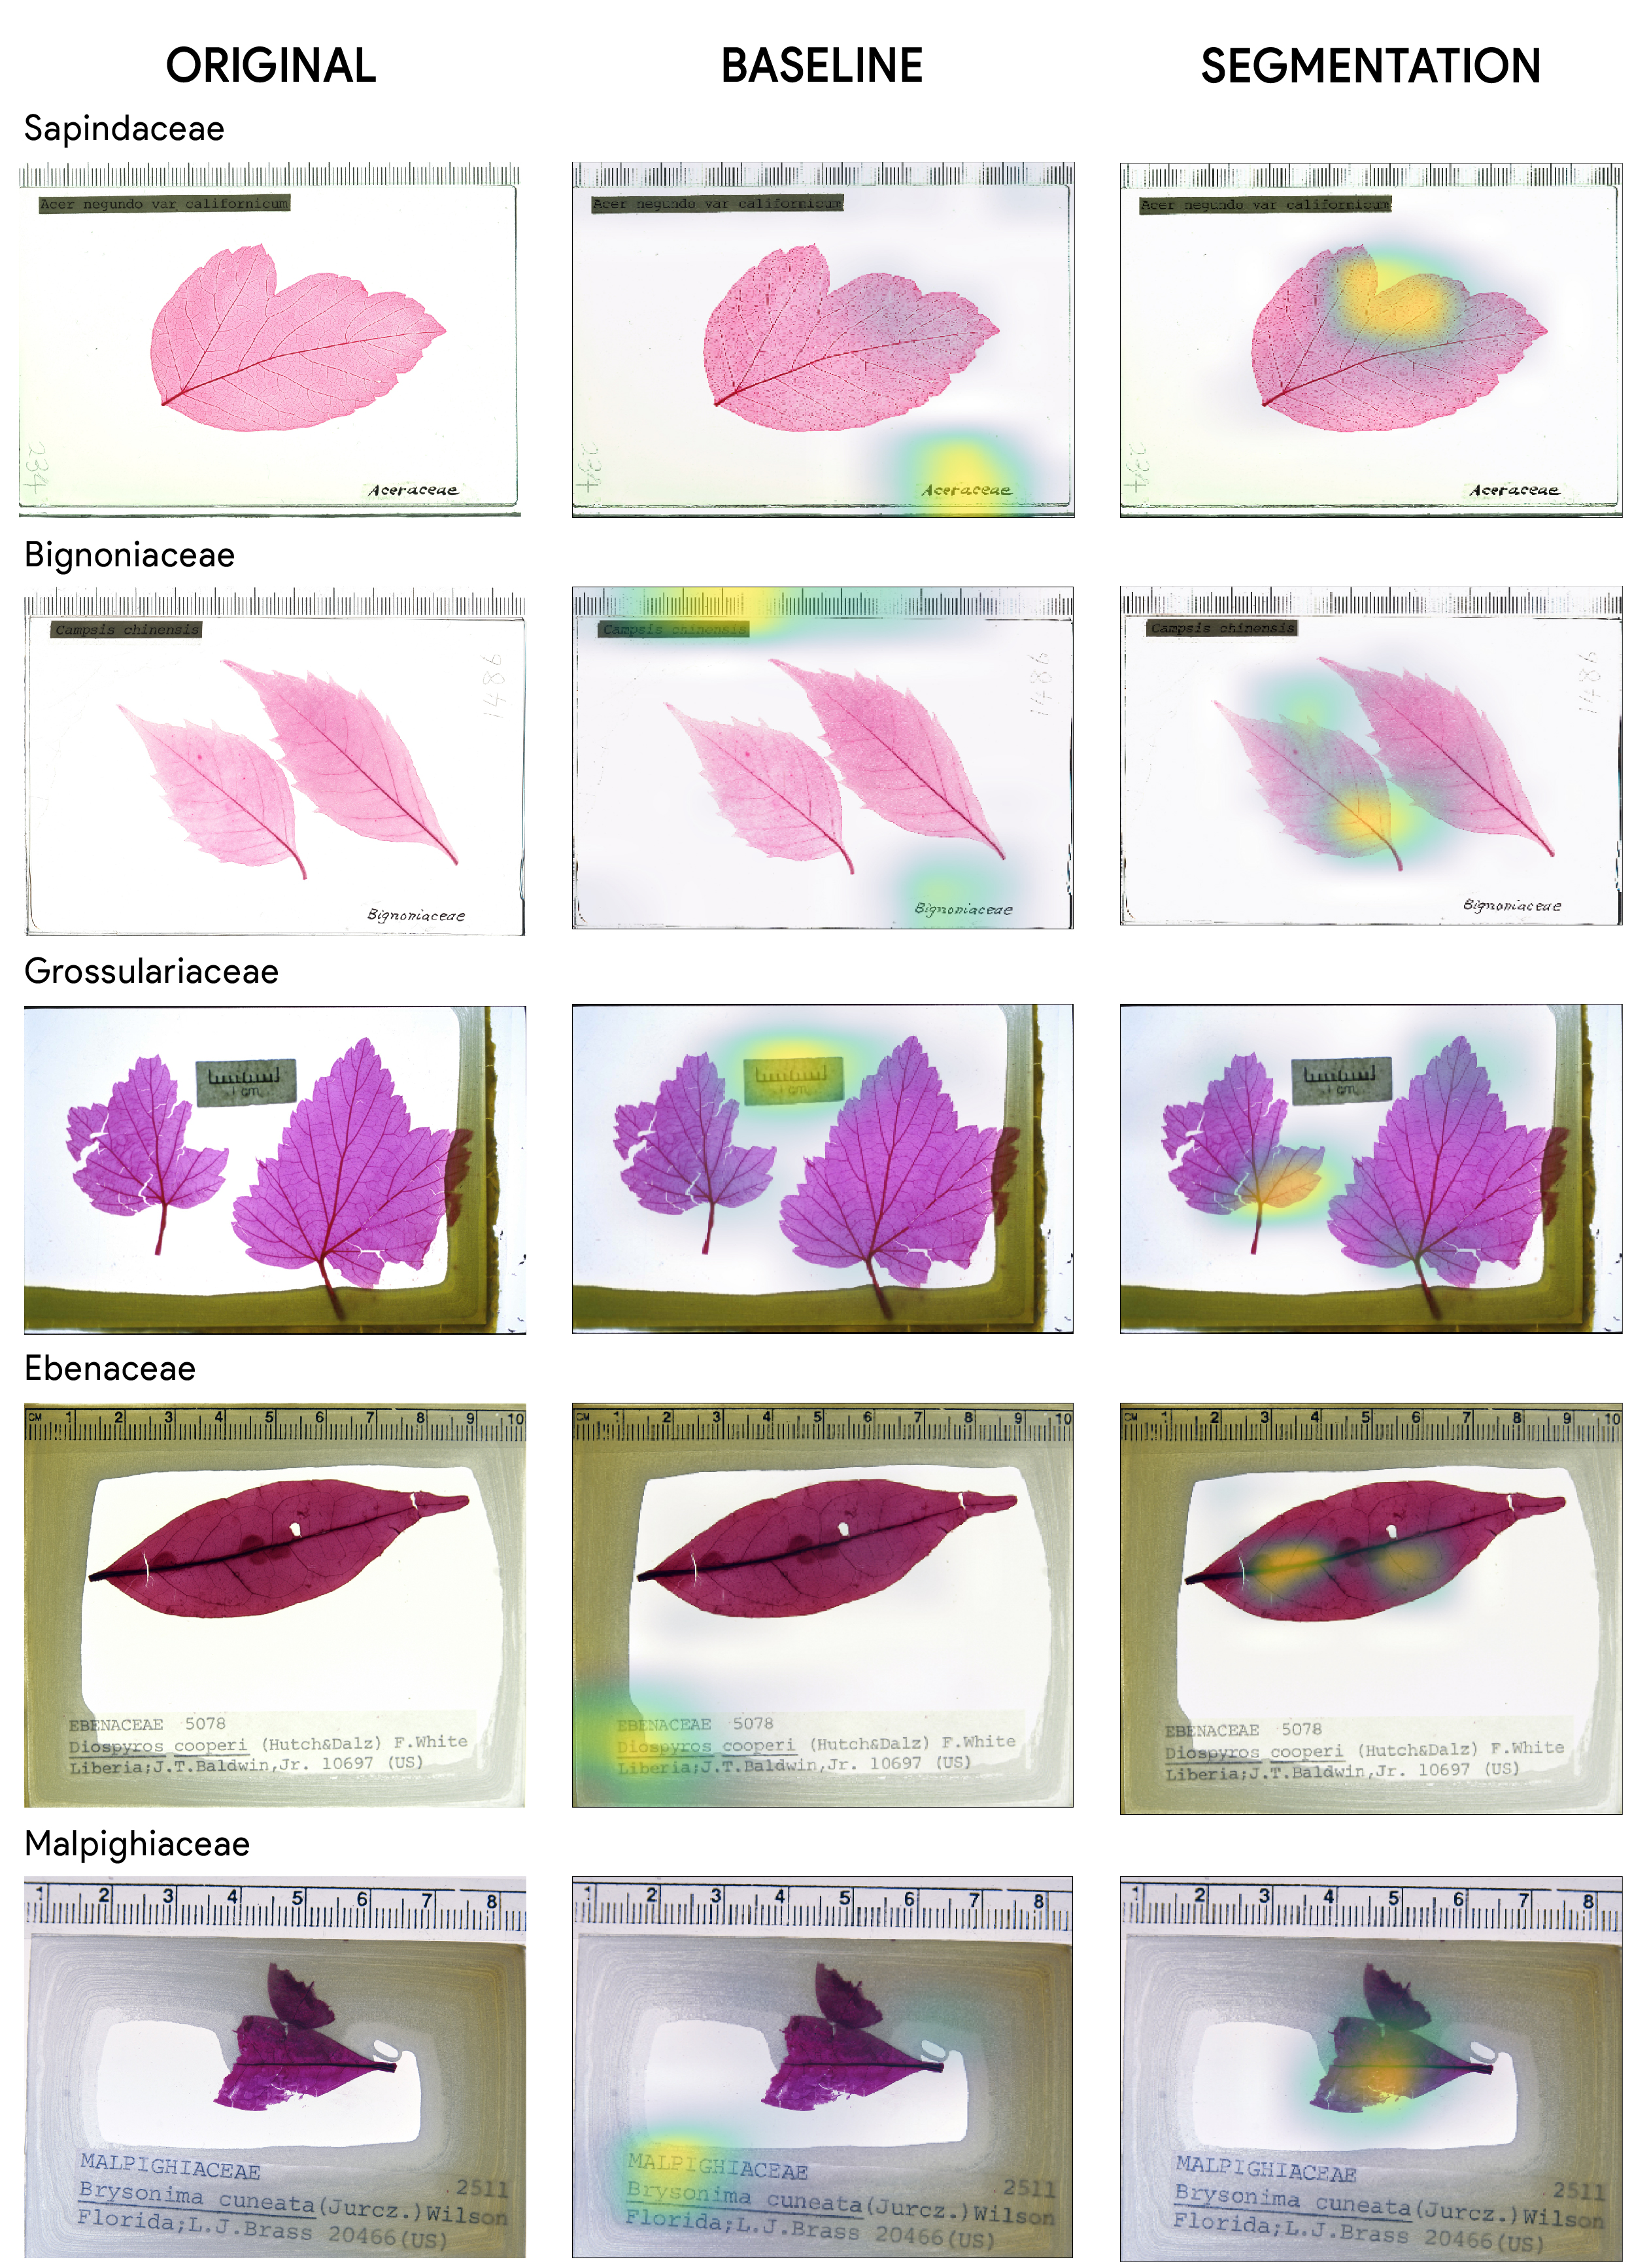
\includegraphics[width=0.6\linewidth]{Figures/SI_Gradcam.jpg}
    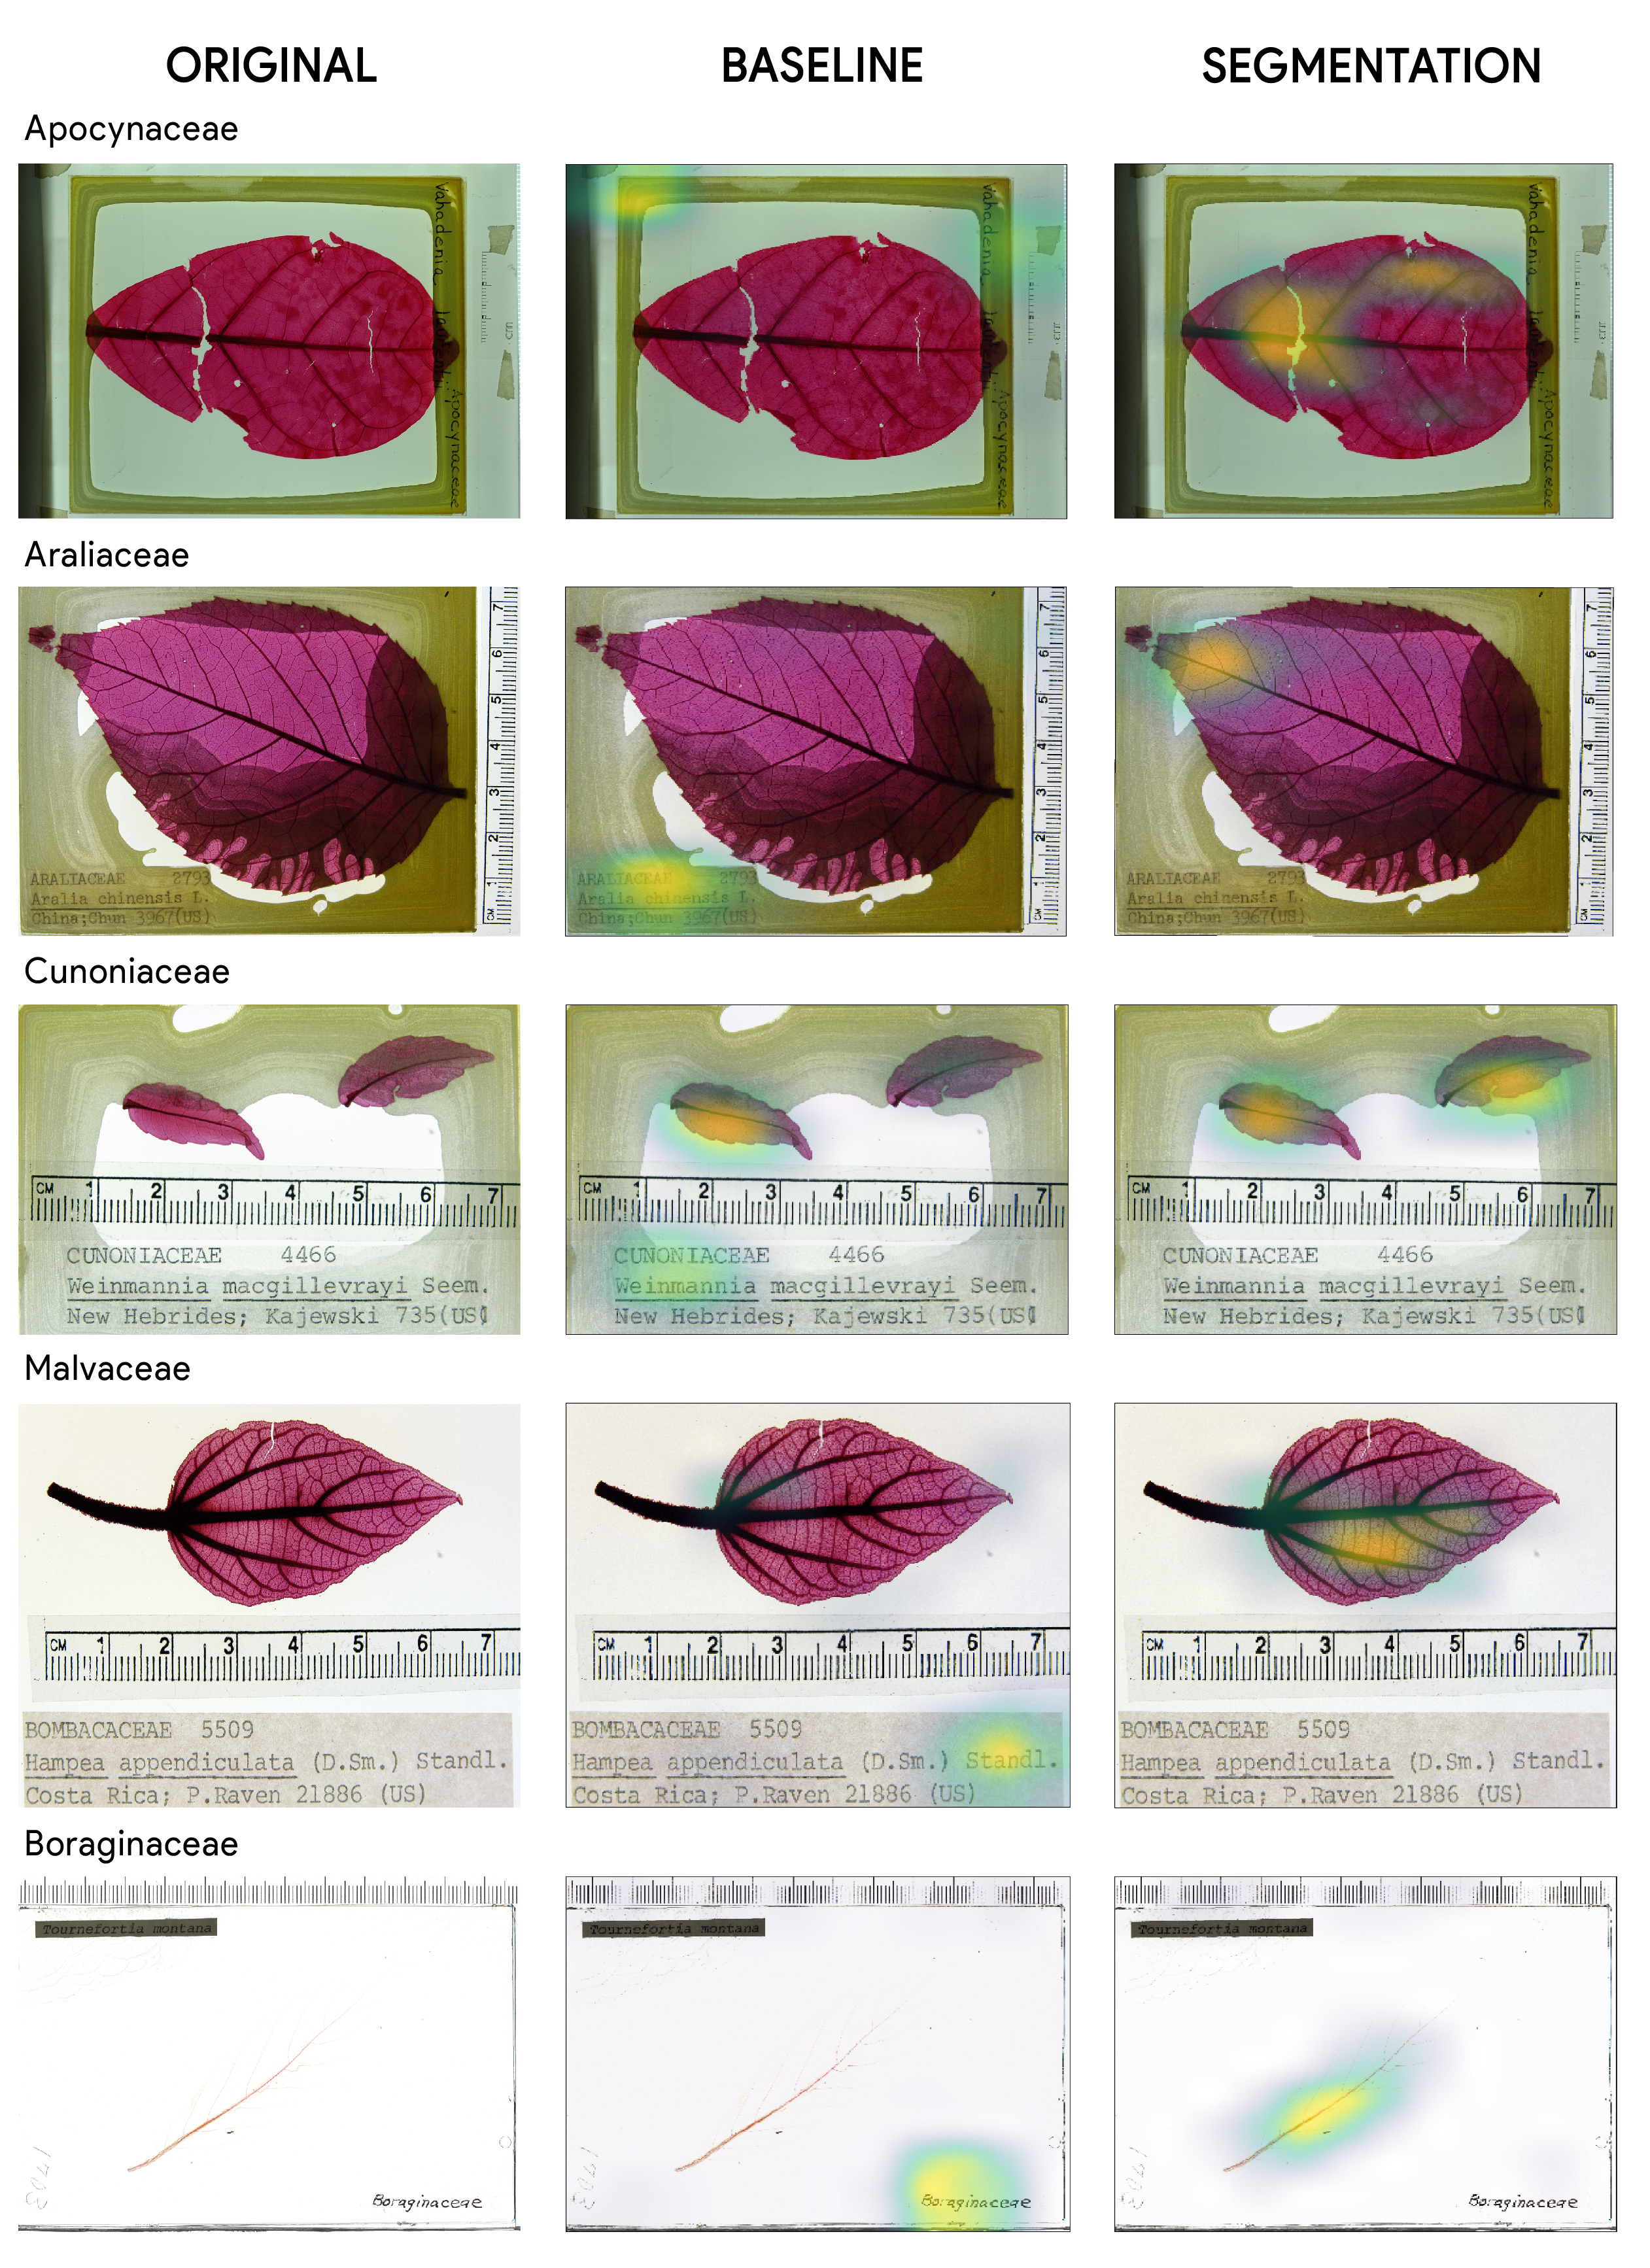
\includegraphics[width=0.6\linewidth]{Figures/SI_Gradcam2.jpg}
    \caption{Attribution map generated using Grad-Cam showing before and after segmentation. For each sample, you will find three columns: Original image on the left, attributions when no segmentation is performed in the middle and in the third column you will find attribution maps from the model trained on segmented leaves reducing the shortcuts used by the model.}\label{fig:attribution_maps}
\end{figure}

\clearpage
\paragraph{System}
Illustration of the system modules. 
\begin{figure}[ht!]
    \centering
    \includegraphics[width=\linewidth]{Figures/Figure_6_v2_system.jpg}
     \caption{Illustration of the System. Top left: Representation of the cleared leaf dataset. Images sampled from 142 families are used as input to the Controlnet to generate synthetic fossils. Bottom left: Representation of the fossil leaf dataset. While the dataset only contains 16 vetted families, we extend the dataset by generating missing fossil families. Middle: Overview of the classification architecture and the ``ControlNet'' prompting approach. Right: Sampling procedure for the triplet loss calculation, within- and cross-domains, taking the furthest positive to bring closer to the anchor and the closest negative to push from the anchor. Bottom right: Illustration of the cycle-consistent approach, where we start from a sample cleared leaf image from the training set and use ControlNet to generate a synthetic fossil. From this synthetic fossil, we then generate a synthetic leaf that is as close as possible to the original sample. }
\label{fig:SI_Full_system}
\end{figure}
% \begin{figure}[ht!]

%     \centering
%     \includegraphics[width=\linewidth]{Figures/GradCAM2.png}
%     \caption{Attribution map generated using GradCAM showing before and after segmentation. For each sample , you will find on the left, attributions when no segmentation is performed, showing that the model relies on non leaf features to classify. On the right you will find same sample , but attribution maps from the model trained on segmented leafs. }
%     \label{fig:attribution_maps}
% \end{figure}

\clearpage
\subsection*{Results of BeIT}
We also investigated a transformer-based architecture, BEiT (BERT pre-training of Image Transformers)~\cite{bao2022beit}, which belongs to a family of vision transformers that have recently achieved state-of-the-art performance across multiple image recognition benchmarks. Unlike convolutional neural networks (CNNs), transformers model long-range dependencies in images via self-attention, enabling them to capture global contextual relationships that can be critical for fine-grained classification tasks. BEiT, in particular, is considered a leading transformer approach, pretrained with a masked image modeling objective inspired by natural language processing. We tested BEiT to evaluate whether transformer-based models could outperform CNNs for fossil leaf classification. However, in our experiments, BEiT showed slightly lower performance than the ResNet-101 baseline presented in the main text (Table~S\ref{tab:beit} summarizes the Top-5 F1-score under the different conditions).

% Note: table counter is reset at line 482, so this is supplementary table 1
\begin{table}[ht!]
\centering
{%
\begin{tabular}{|c|c|c|c|}
\hline
Condition &
  \begin{tabular}[c]{@{}c@{}}Top 5\\ Lower Bound\end{tabular} &
  \begin{tabular}[c]{@{}c@{}}Top 5 \\ Upper Bound\end{tabular} &
  \#families \\ \hline
Unsegmented                                                   & 4.21\% & 64.3\% & 142 \\ \hline
Segmented                                                     & 6.21\% & 65.1\% & 142 \\ \hline
\begin{tabular}[c]{@{}c@{}}Triplet +\\ Segmented\end{tabular} & 21.4\% & 72\%   & 142 \\ \hline
\begin{tabular}[c]{@{}c@{}}Triplet + \\ Segmented +\\ Synthetic Fossils\end{tabular} &
  \textbf{75.1\%} &
  \textbf{86.4\%} &
  142 \\ \hline

\end{tabular}%
}
\caption{BEiT classification results under the different conditions studied.}
\label{tab:beit}
\end{table}

\paragraph{Details for Training}
We use a Large Memory IBM Node with 4 V100 GPUs and 1TB of RAM with fast interconnect between RAM and GPU. One GPU was exclusively hosting the SAM model trained for image silhouette detection, while the other three hosted the Control Net running on Stable Diffusion 2.1 and the classification model. The batch size was 64 with a total resolution of 512x512.  

\subsection*{Additional Concepts}
Find examples of more concepts that our model finds below, and please visit our website \url{https://fel-thomas.github.io/Leaf-Lens/} for an exhaustive list of concepts.  
\begin{figure}
    \centering
    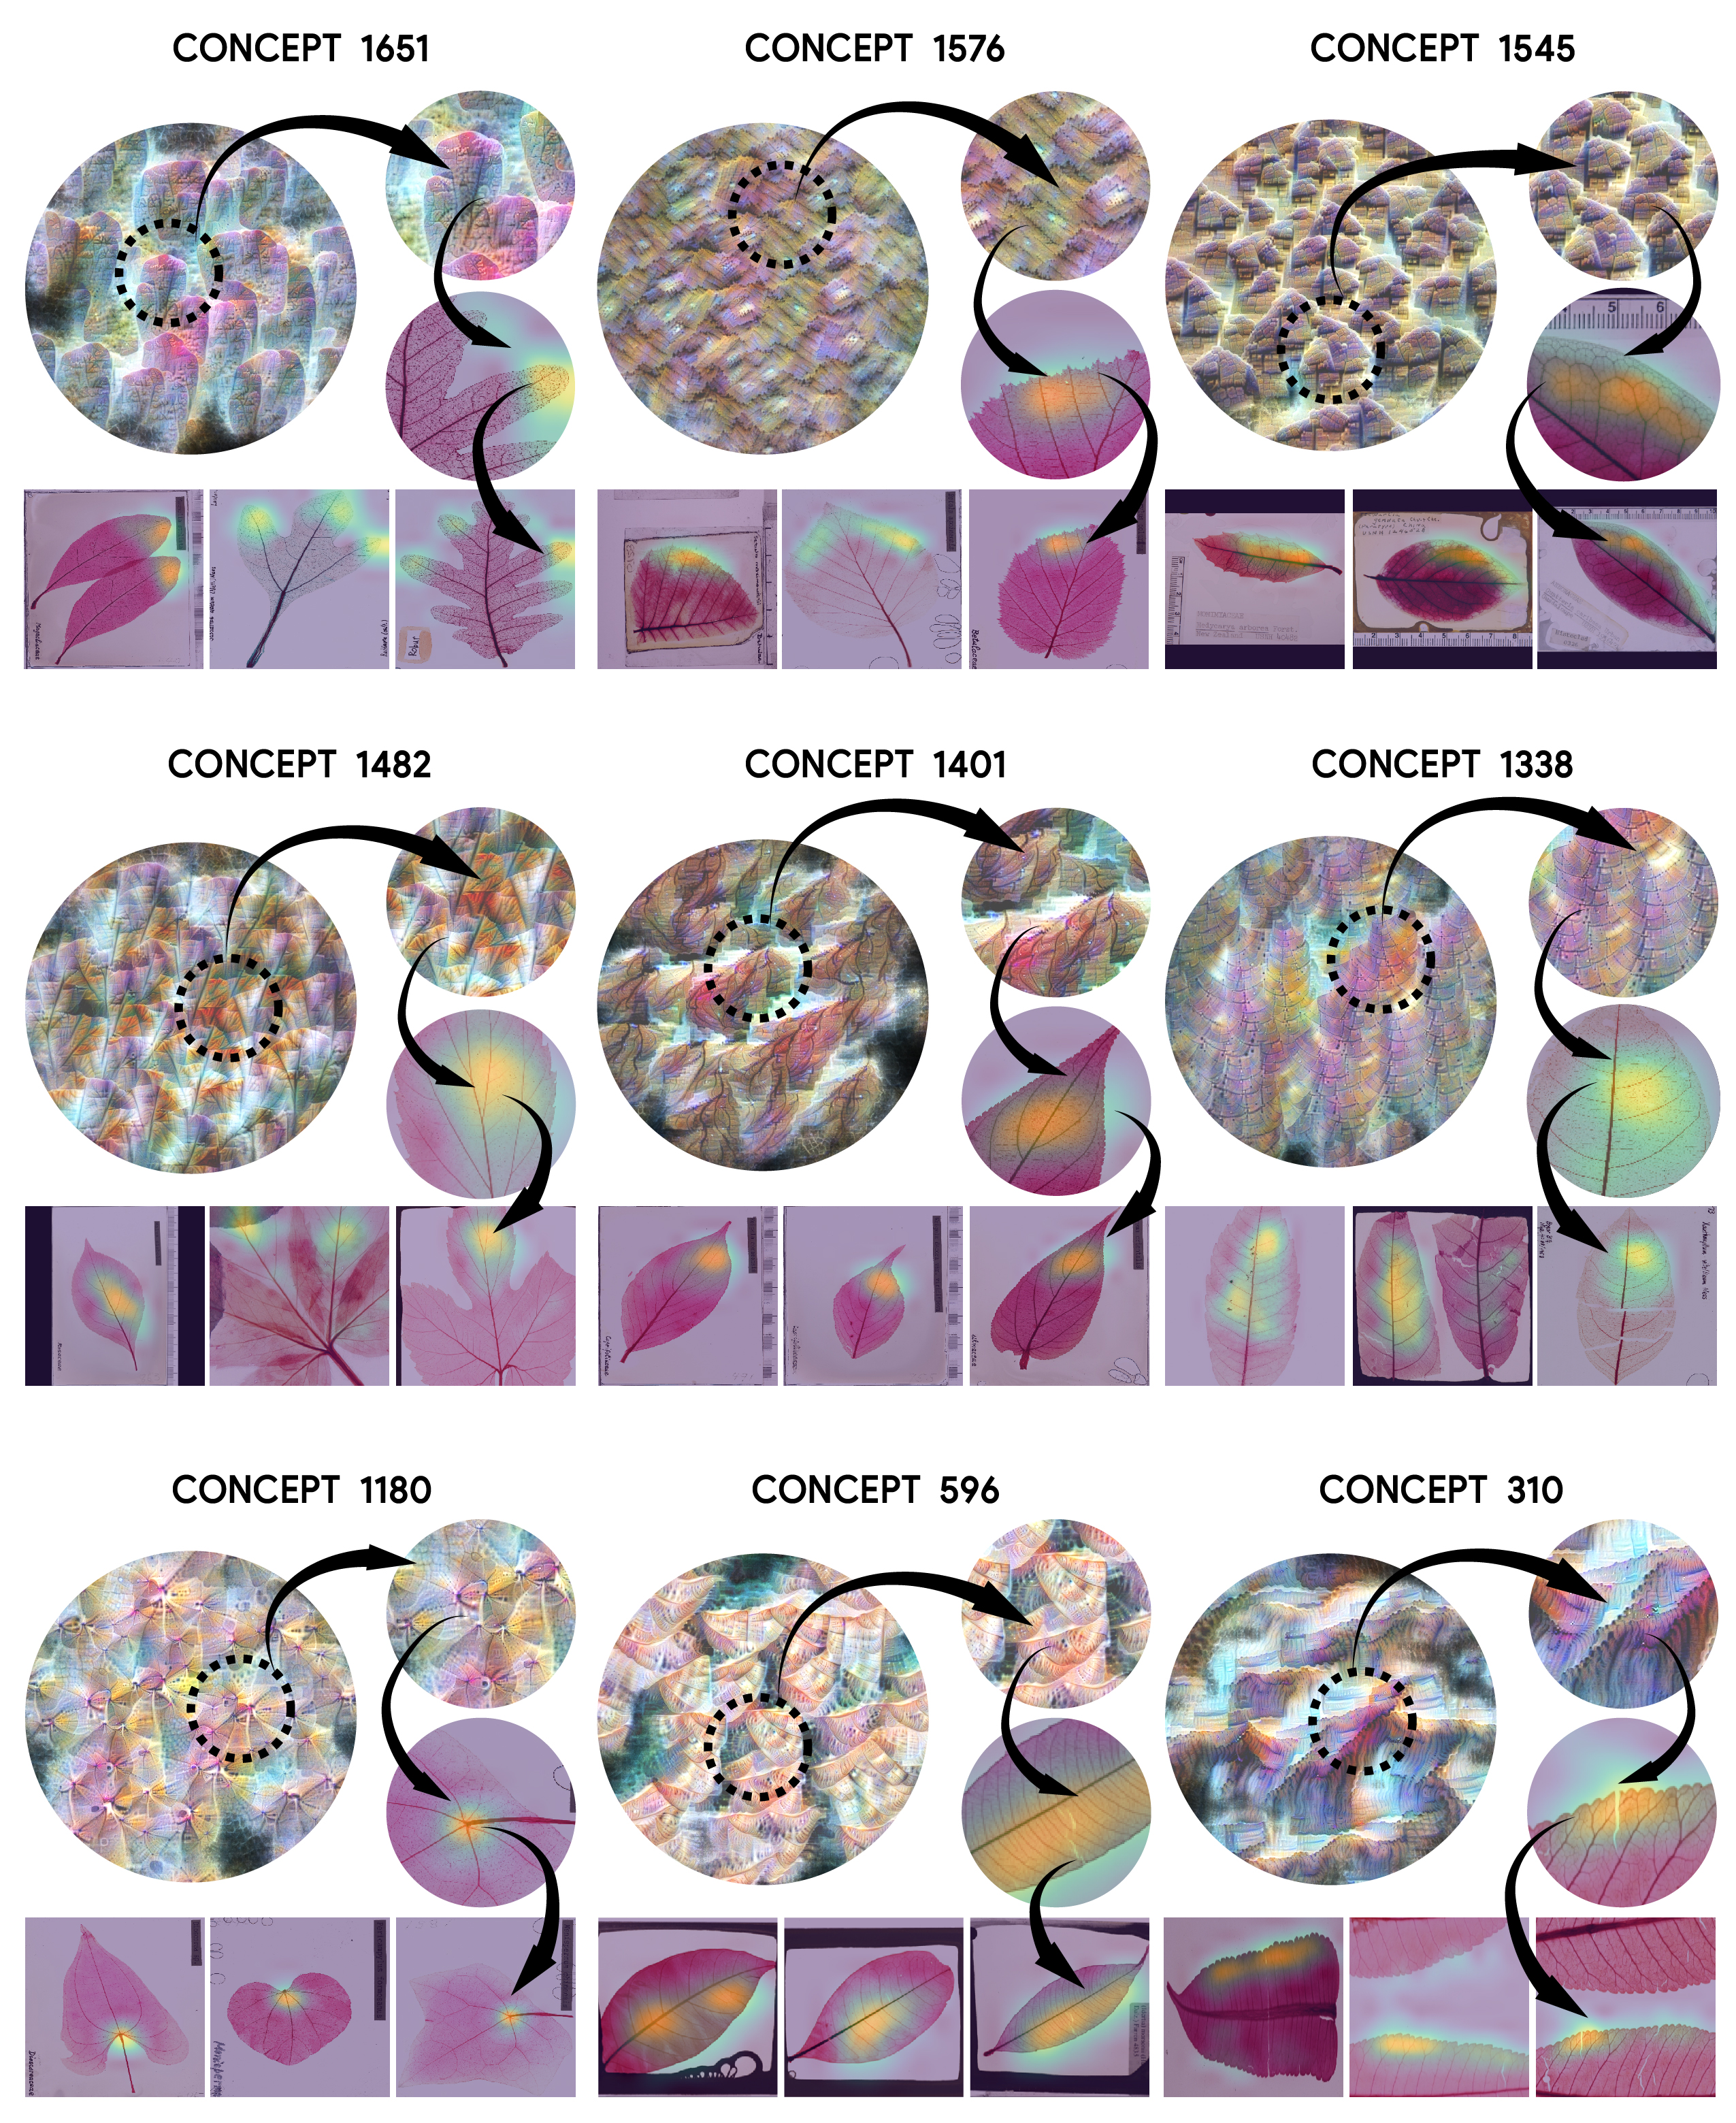
\includegraphics[width=\linewidth]{Figures/SI_6A.jpg}
    
    \caption{Examples of more concepts used by the model. }
    % Footnote moved outside caption

\label{fig:SI_concepts}
\end{figure}


\begin{figure}
    \centering
    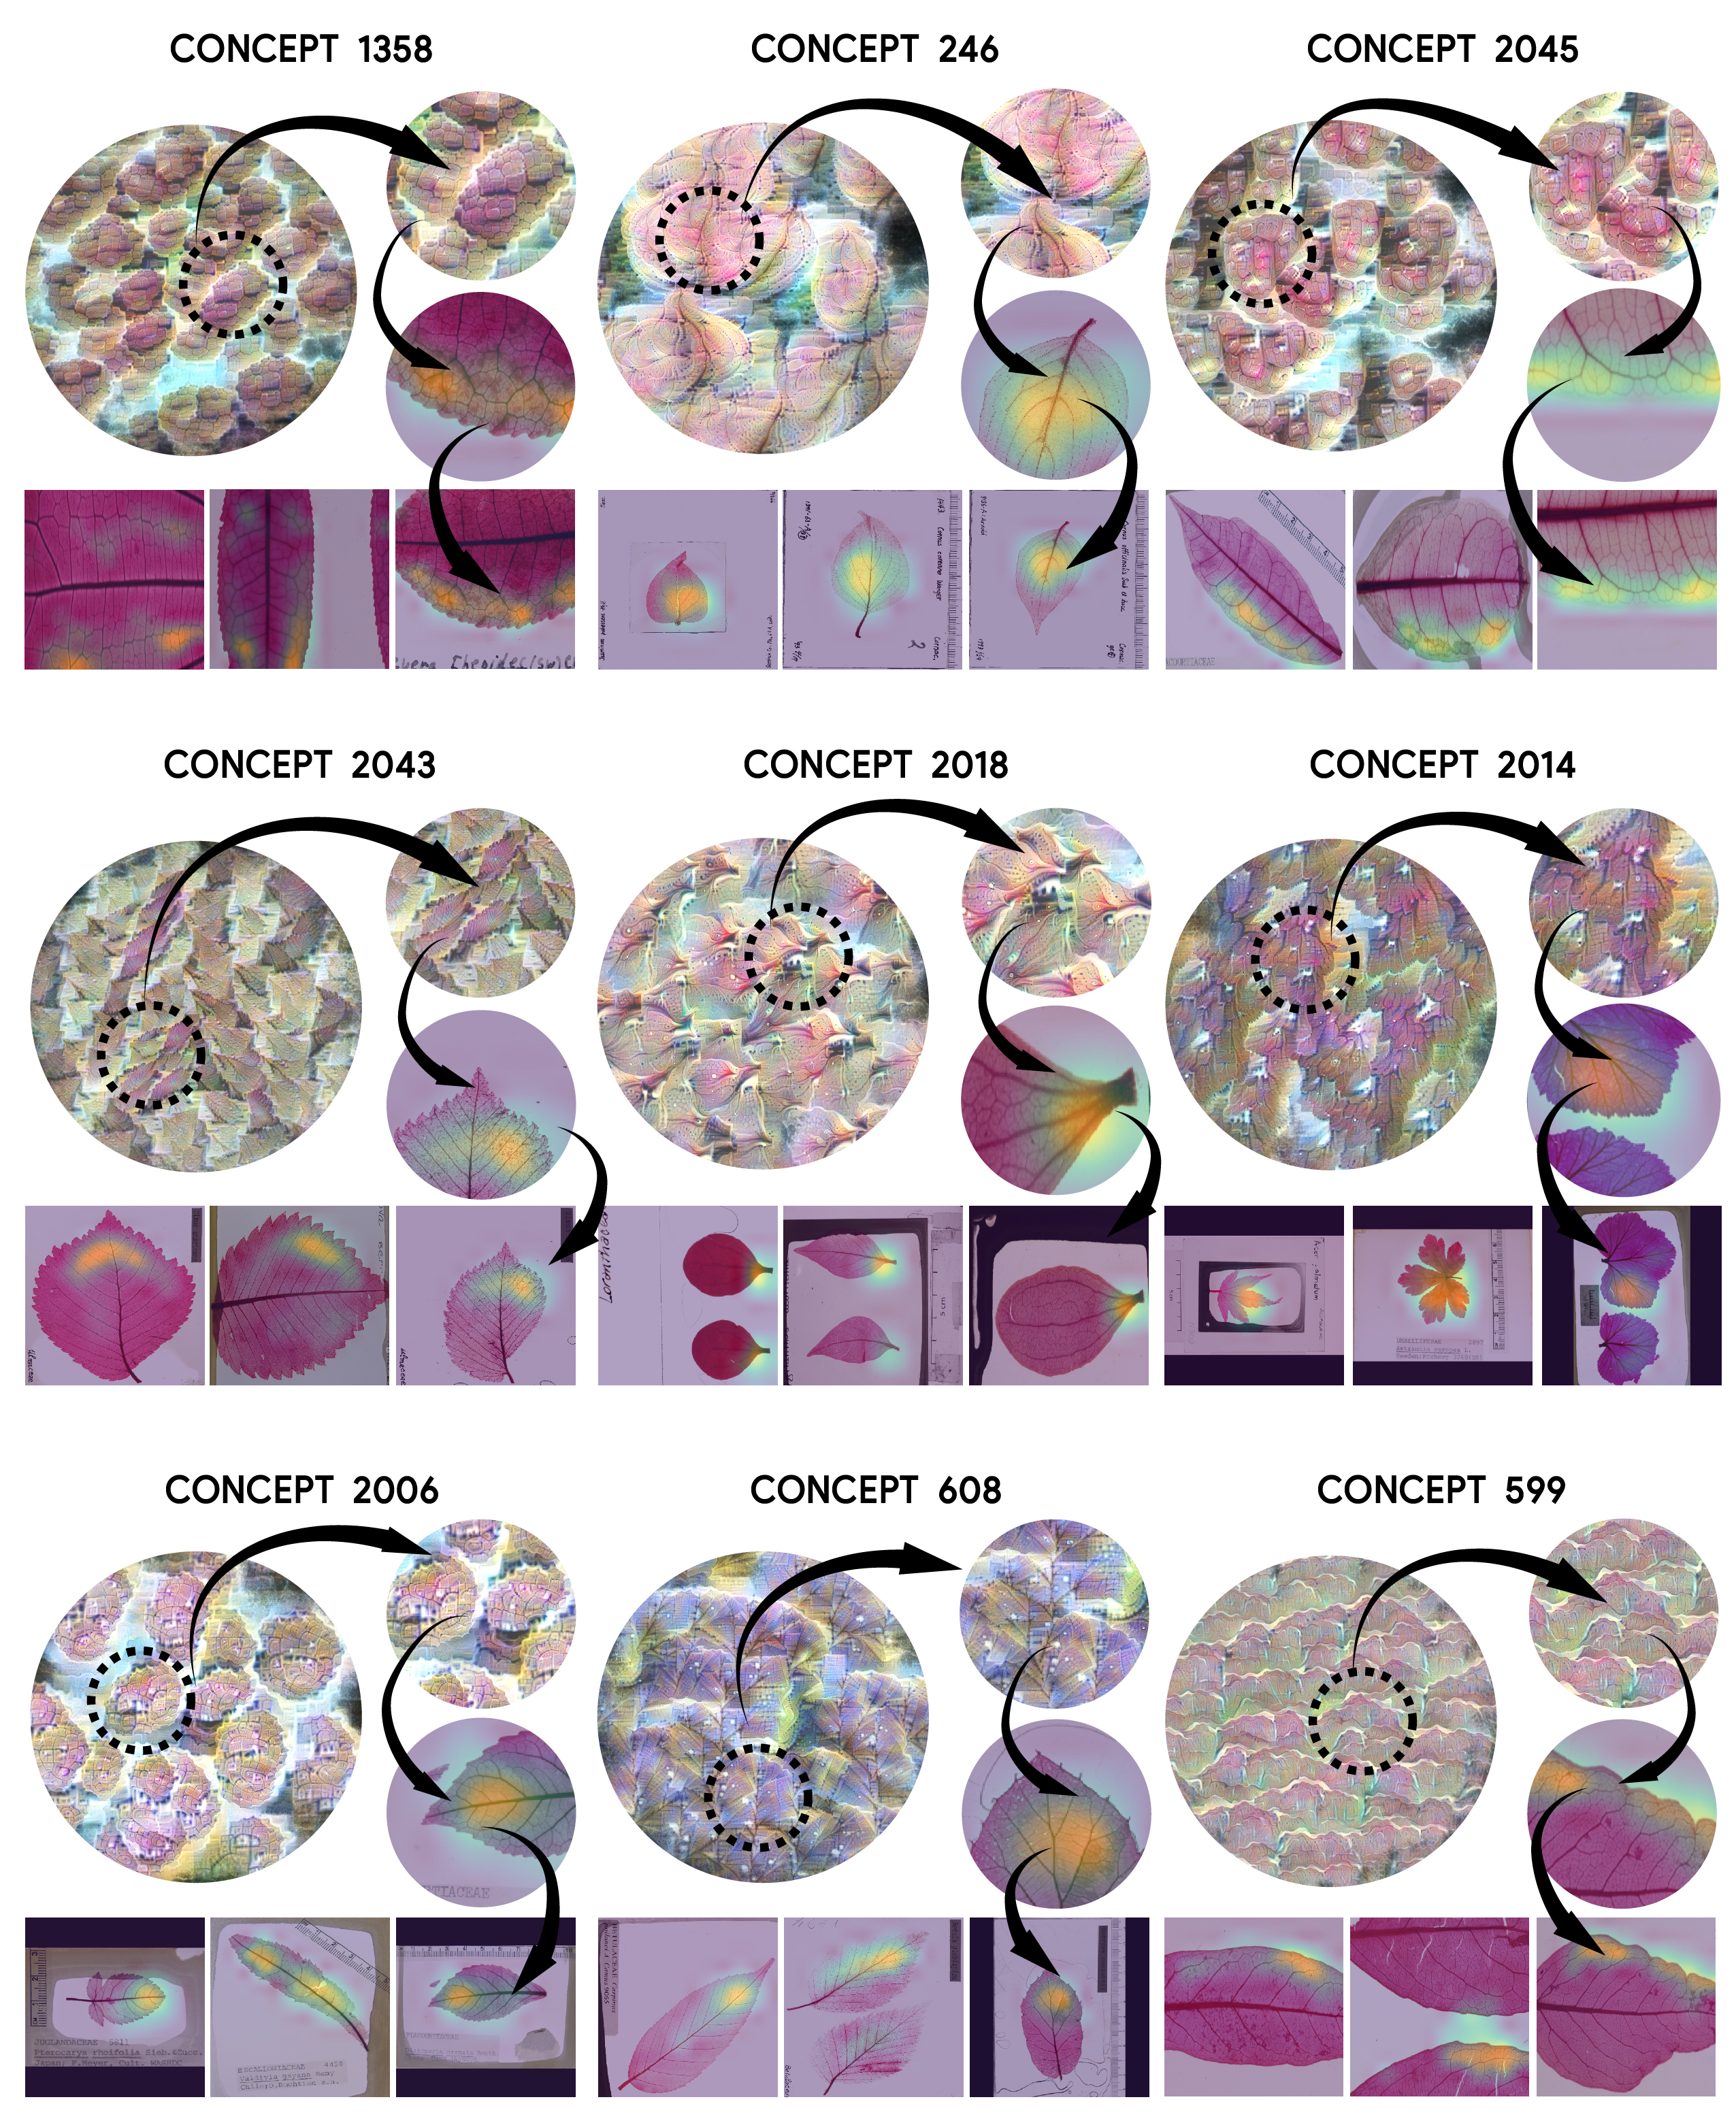
\includegraphics[width=\linewidth]{Figures/SI_6B.jpg}
    
    \caption{Additional examples  of concepts used by the model.}
    % Footnote moved outside caption

\label{fig:SI_concepts2}
\end{figure}

% \bibliographystyle{sn-mathphys}
% \bibliography{sn-bibliography}% common bib file

%% if required, the content of .bbl file can be included here once bbl is generated
%%\input sn-article.bbl

\end{oldappendices}
\end{document}